% !TEX root = ../report.tex
\section*{Differences Between Semesters} \label{sec:experiments}
\addcontentsline{toc}{section}{Differences Between Semesters}
In this section we will discuss some of the differences between the first and second semester of our master thesis special. 

\subsection*{Pull Techniques}
The techniques used in the two studies this semester were twice the number of techniques we experimented with last semester which only compared 4 push techniques.
The studies this semester also include the pull direction from the large display to the phone.
\Cref{fig:pullTechniques} shows the figures for all the pull techniques. 
We did not add them to the paper since we felt that we explained the pull techniques sufficienctly with the push technique figures.
If we had added them, they would have taken a lot of extra space, which we wanted to use for other things. 


\begin{figure}[H]
	\subfloat[\grab \pull technique]{
		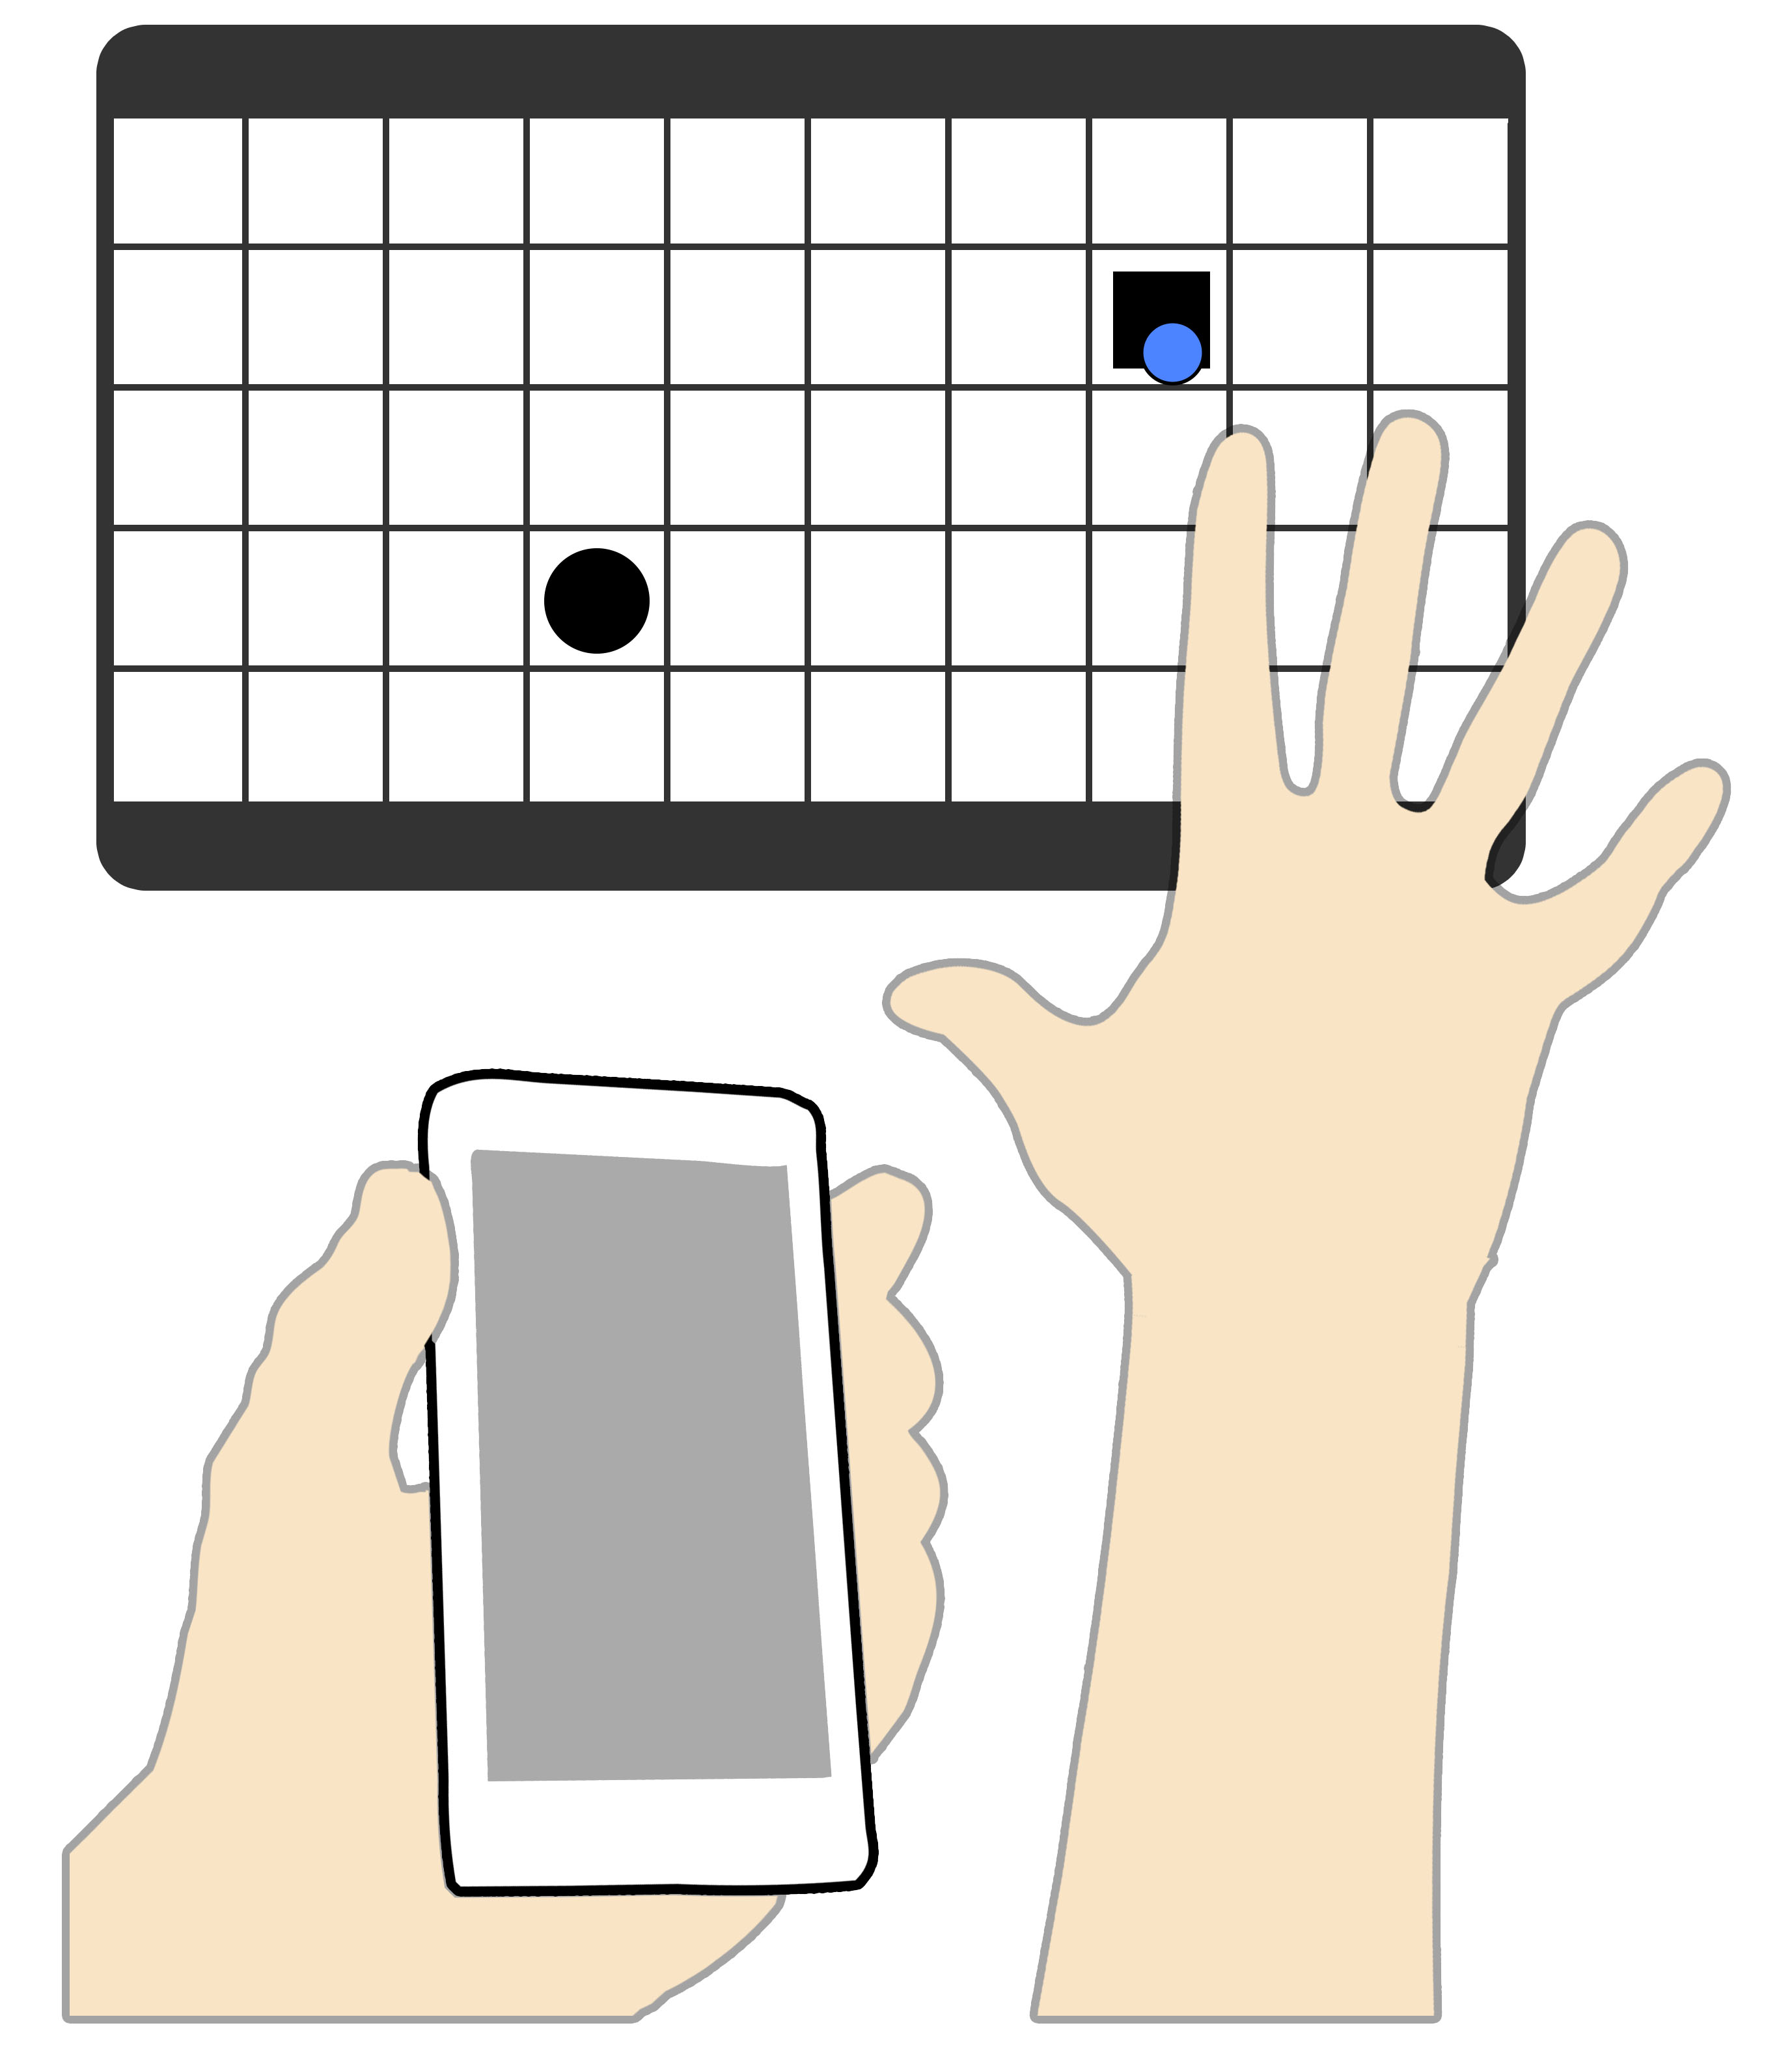
\includegraphics[width = 0.16\columnwidth]{images/techniques/grabPull1.jpg}\label{fig:grabPull1}
		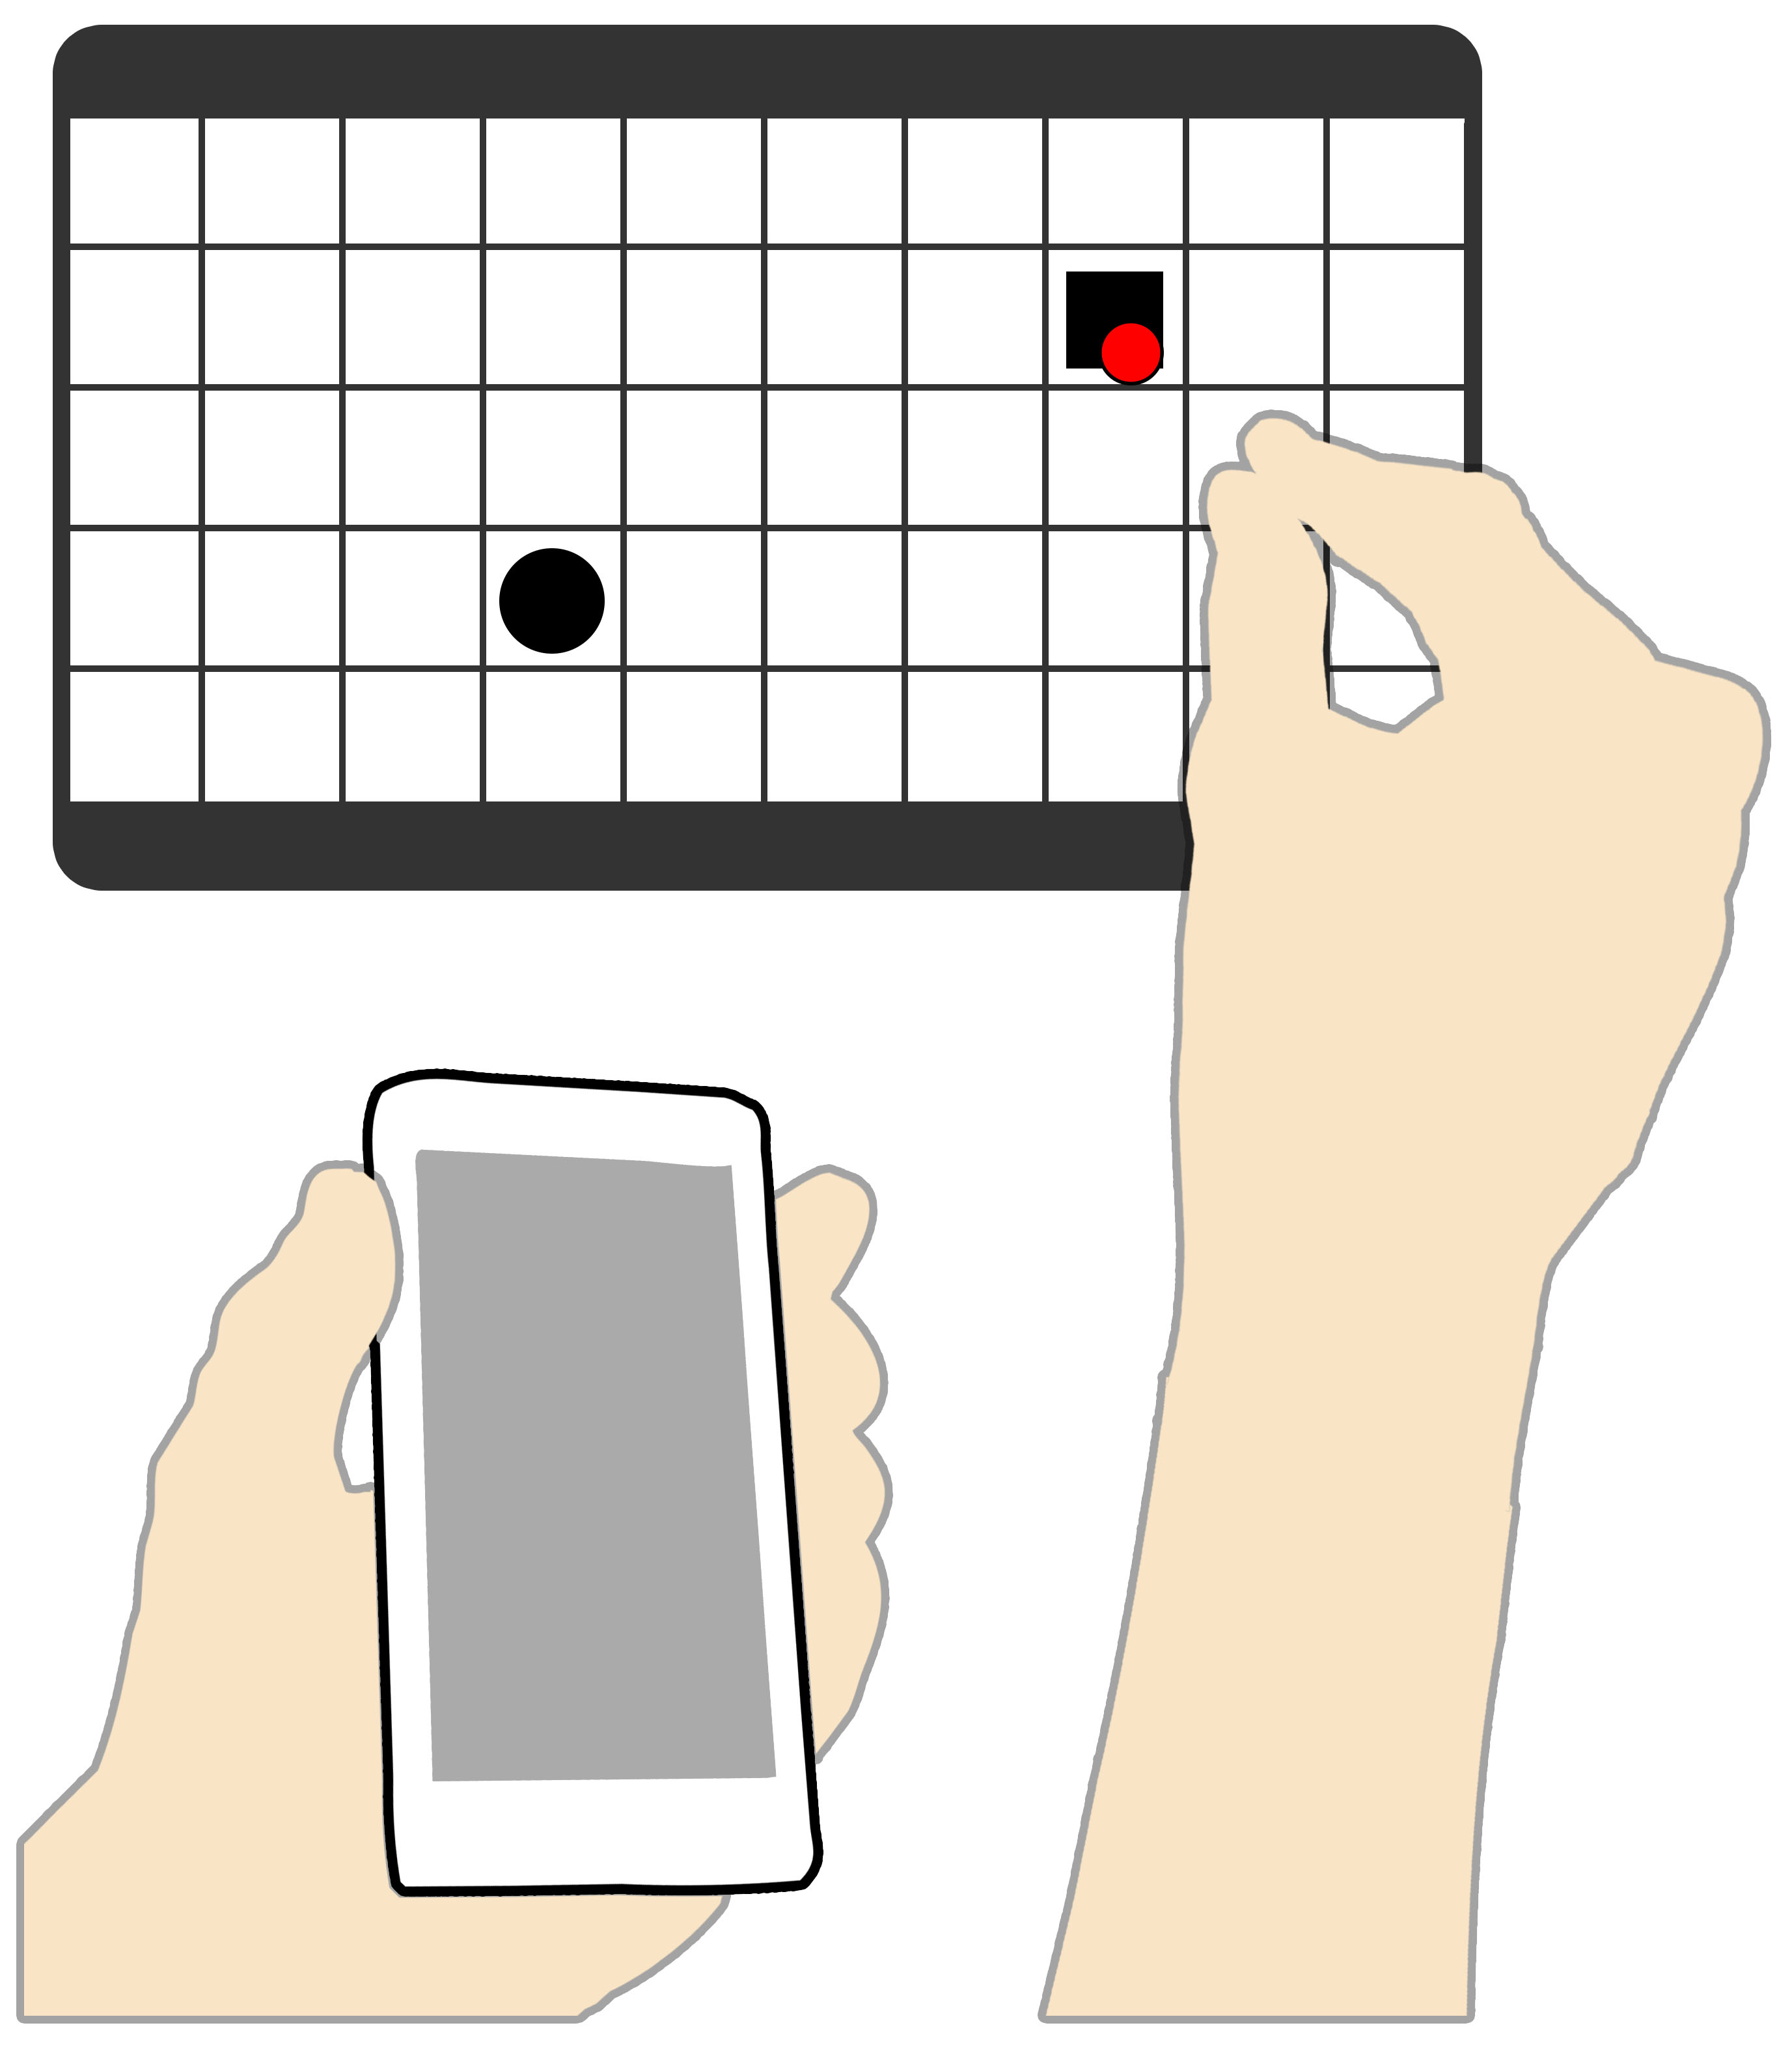
\includegraphics[width = 0.16\columnwidth]{images/techniques/grabPull2.jpg}\label{fig:grabPull2}
		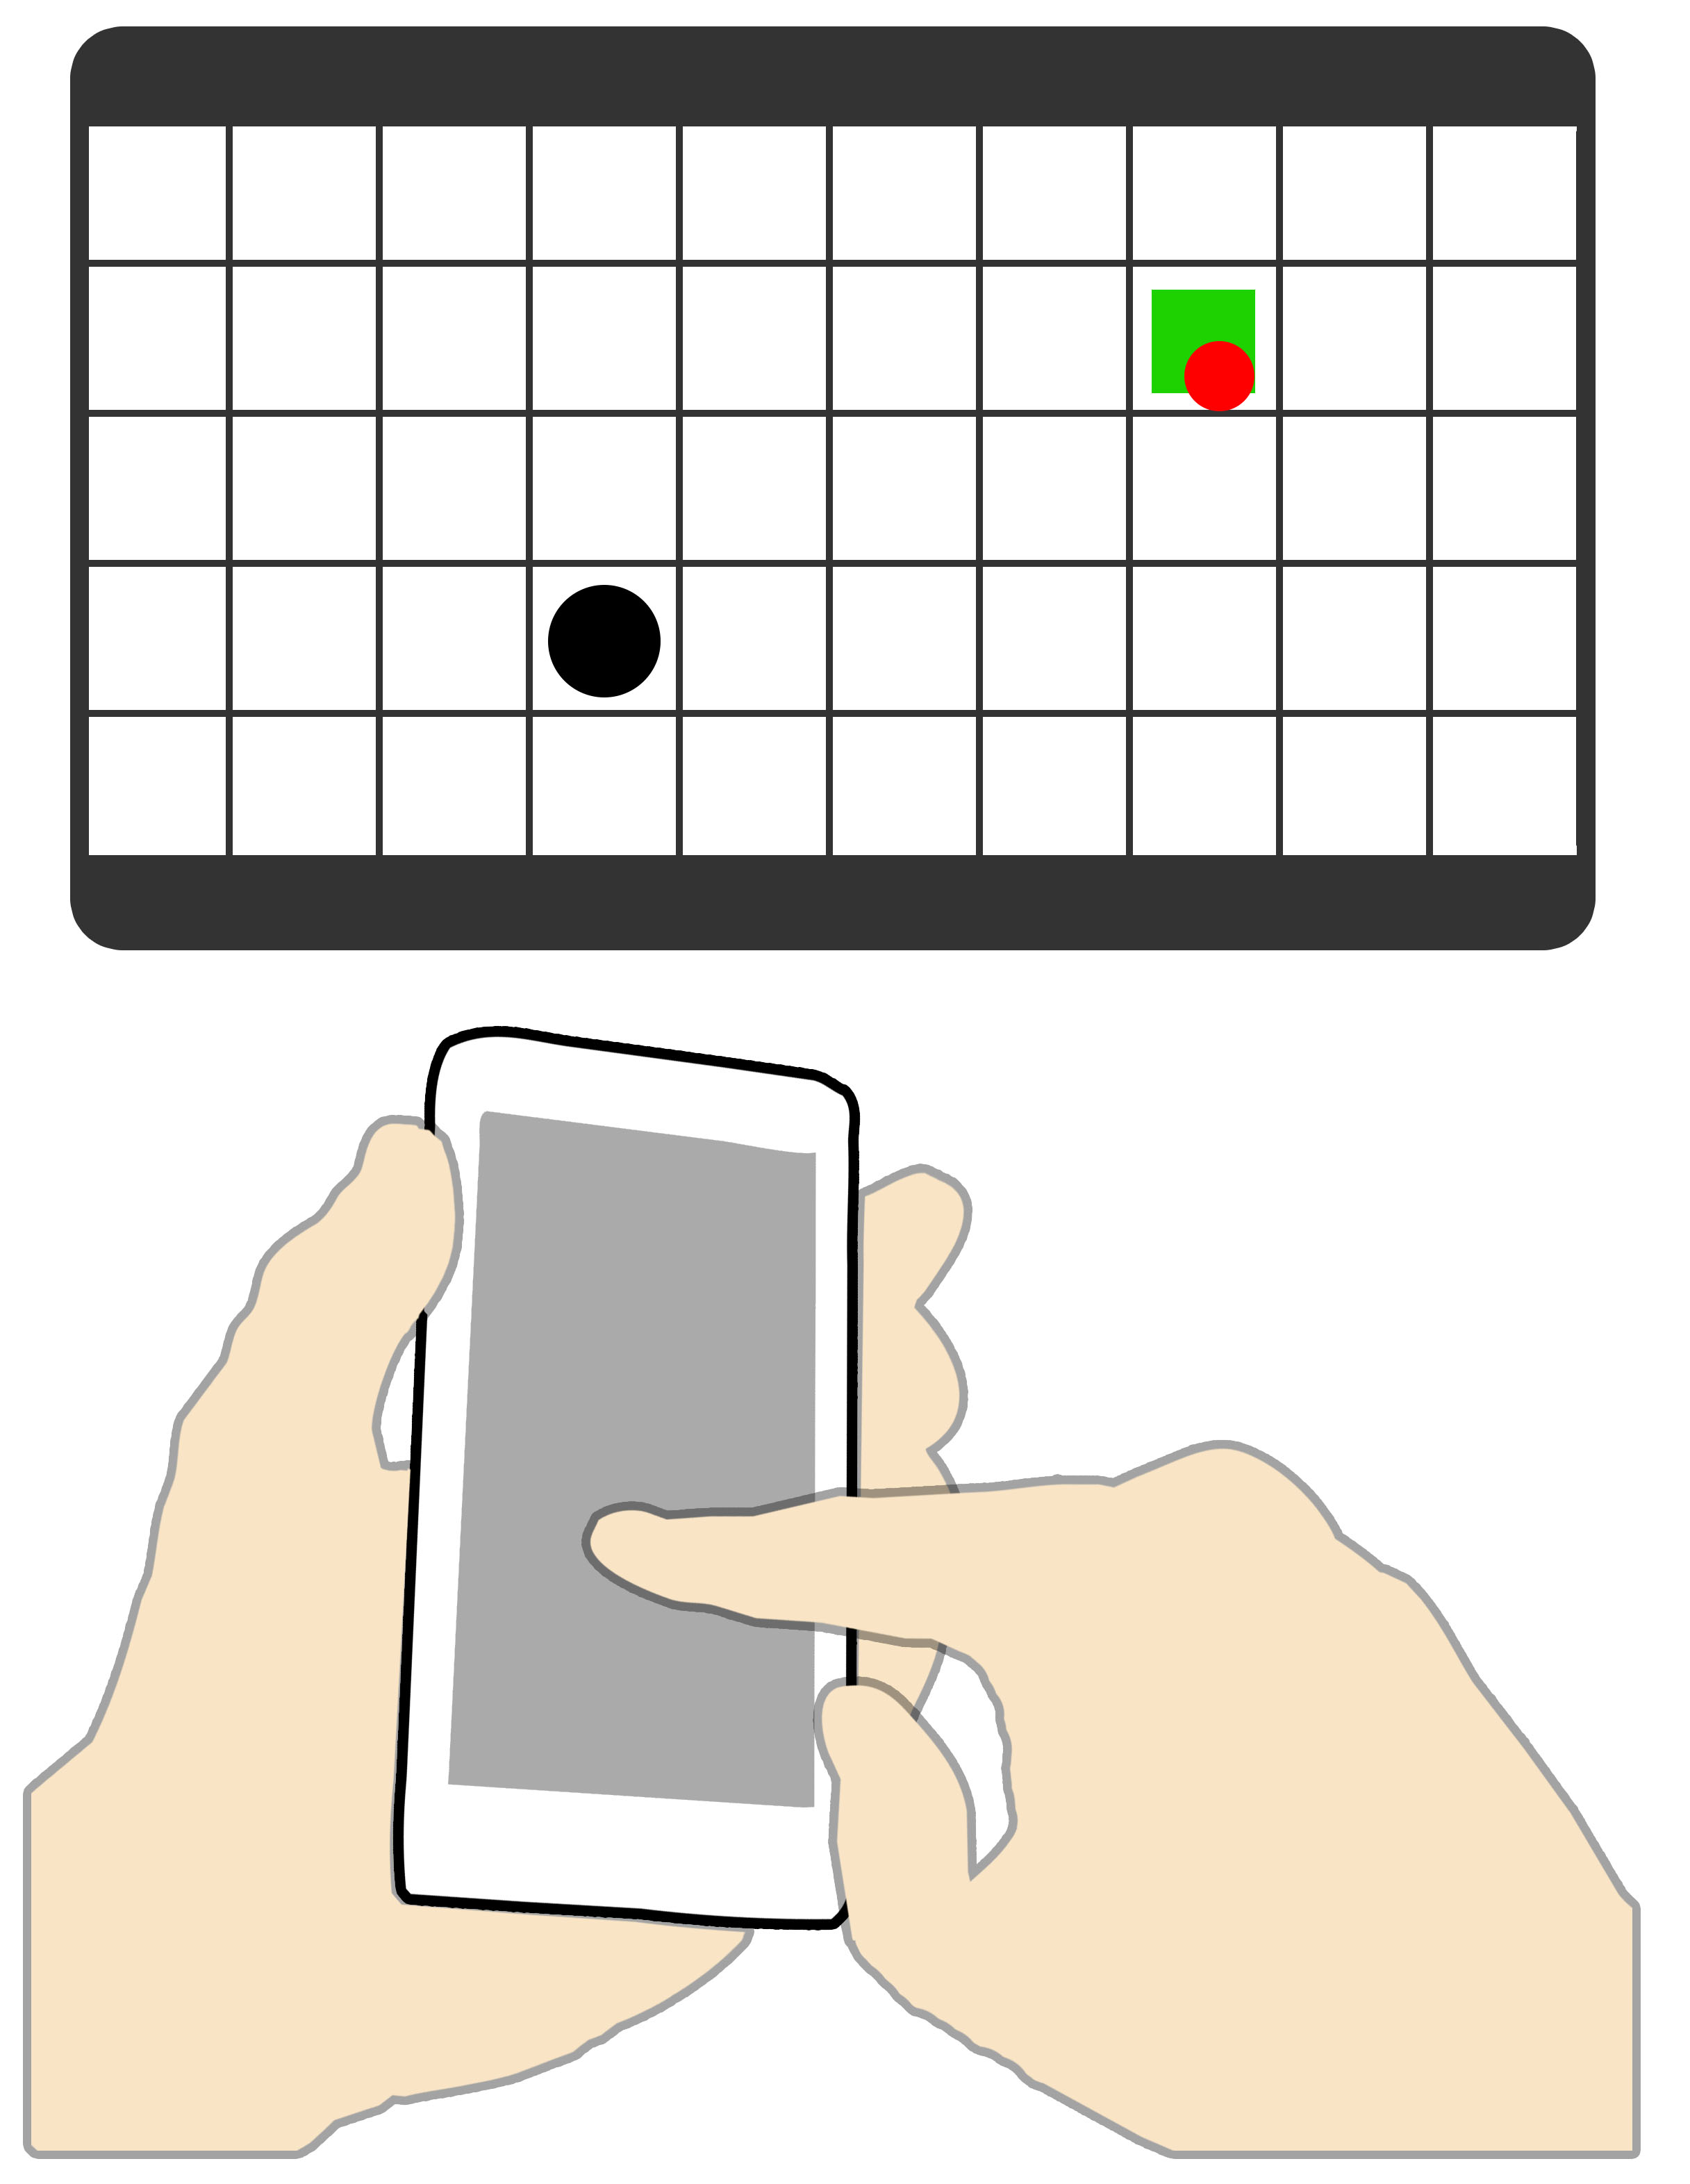
\includegraphics[width = 0.16\columnwidth]{images/techniques/grabPull3.jpg}\label{fig:grabPull3}}
	\subfloat[\swipe \pull technique]{
		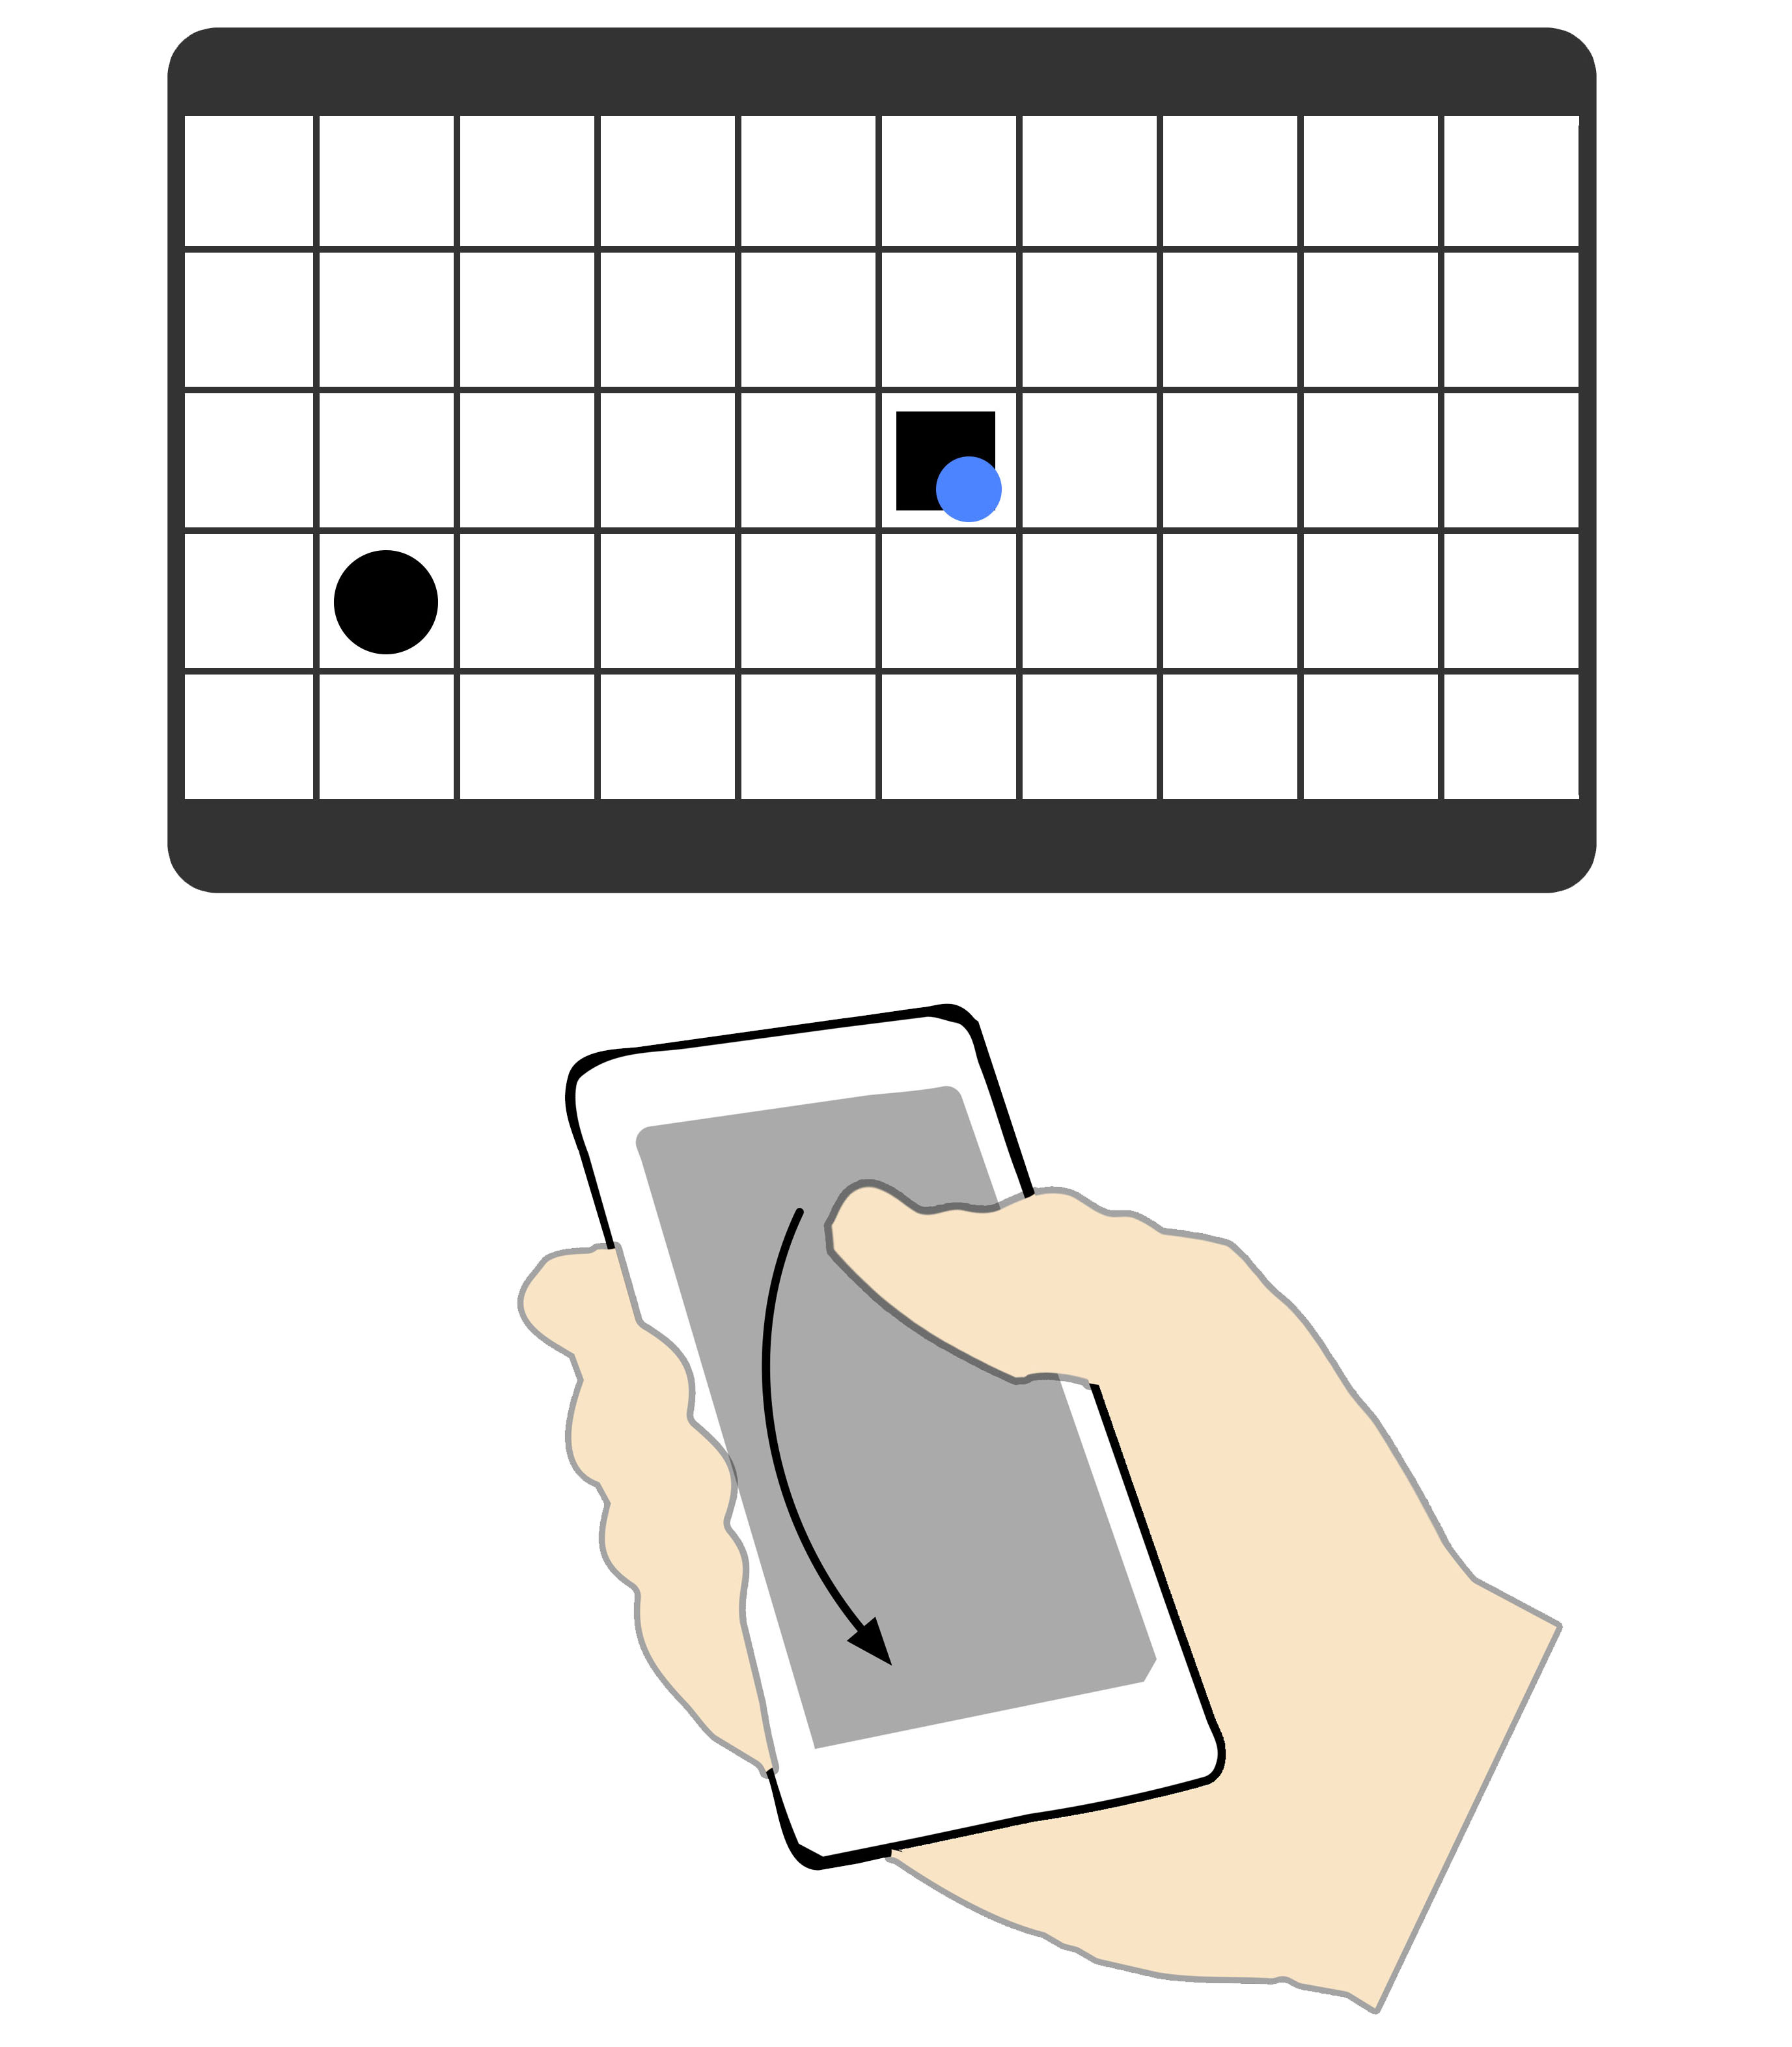
\includegraphics[width = 0.16\columnwidth]{images/techniques/swipePull1.jpg}\label{fig:swipePull1}
		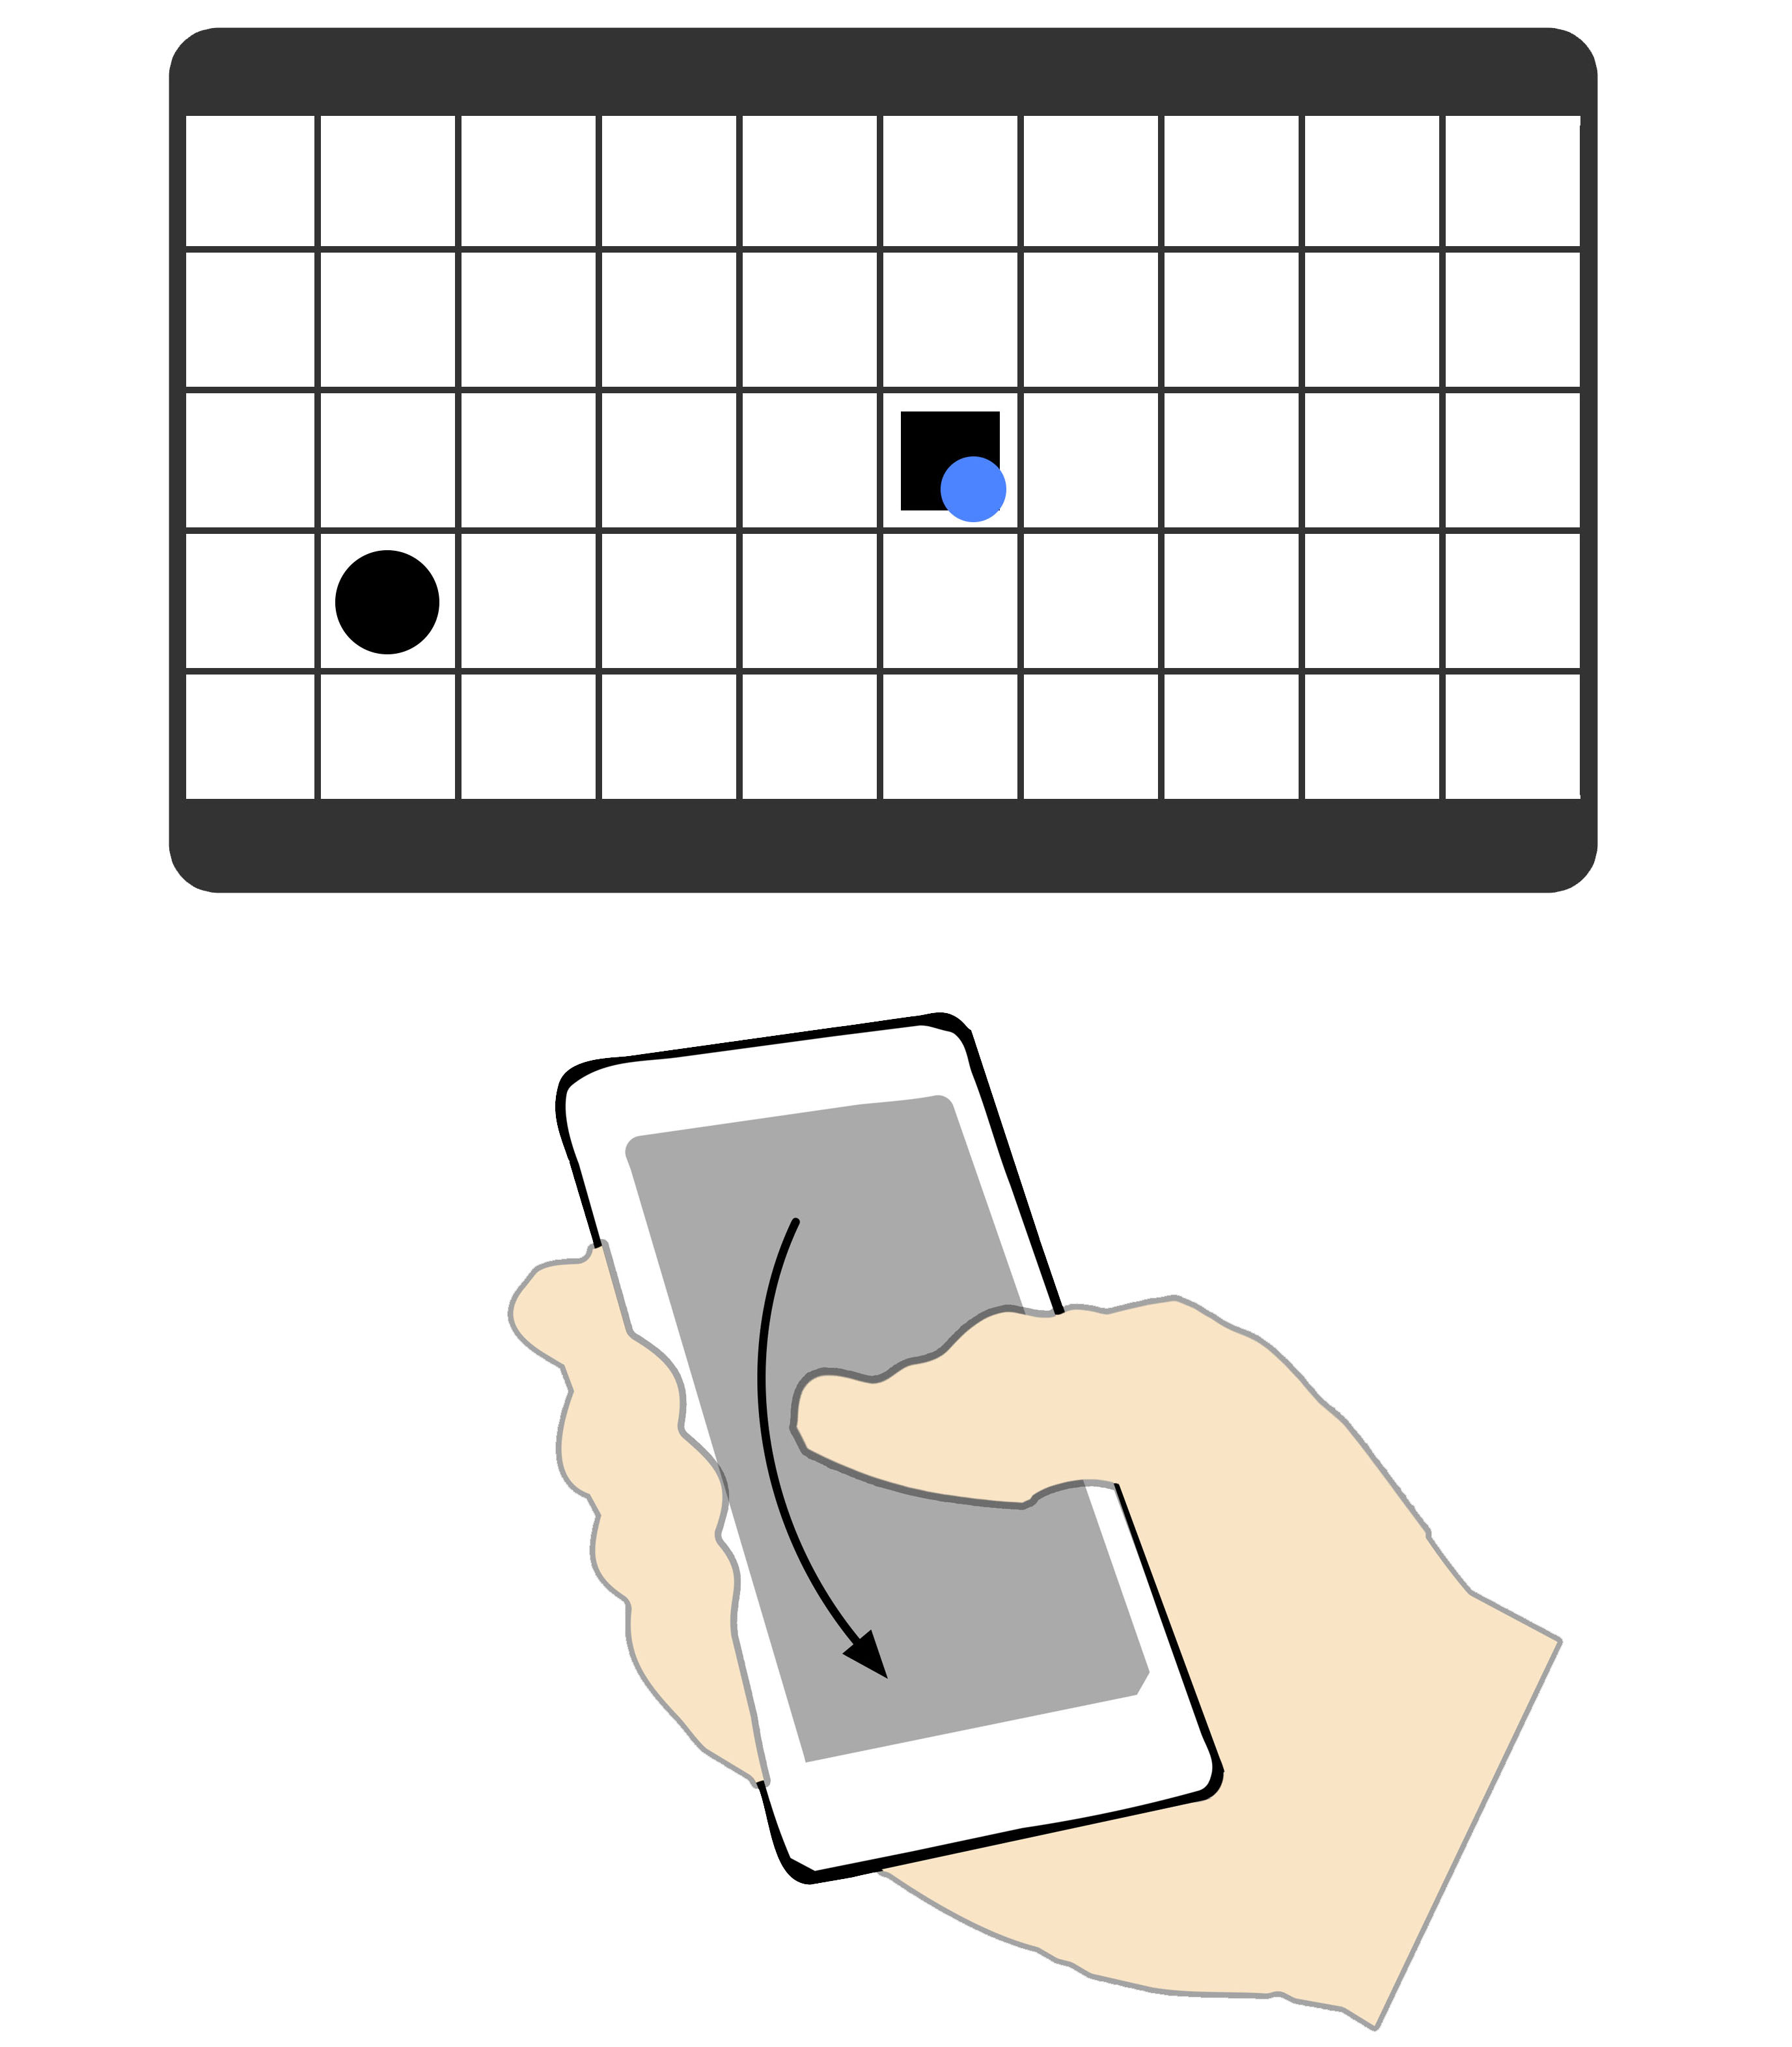
\includegraphics[width = 0.16\columnwidth]{images/techniques/swipePull2.jpg}\label{fig:swipePull2}
		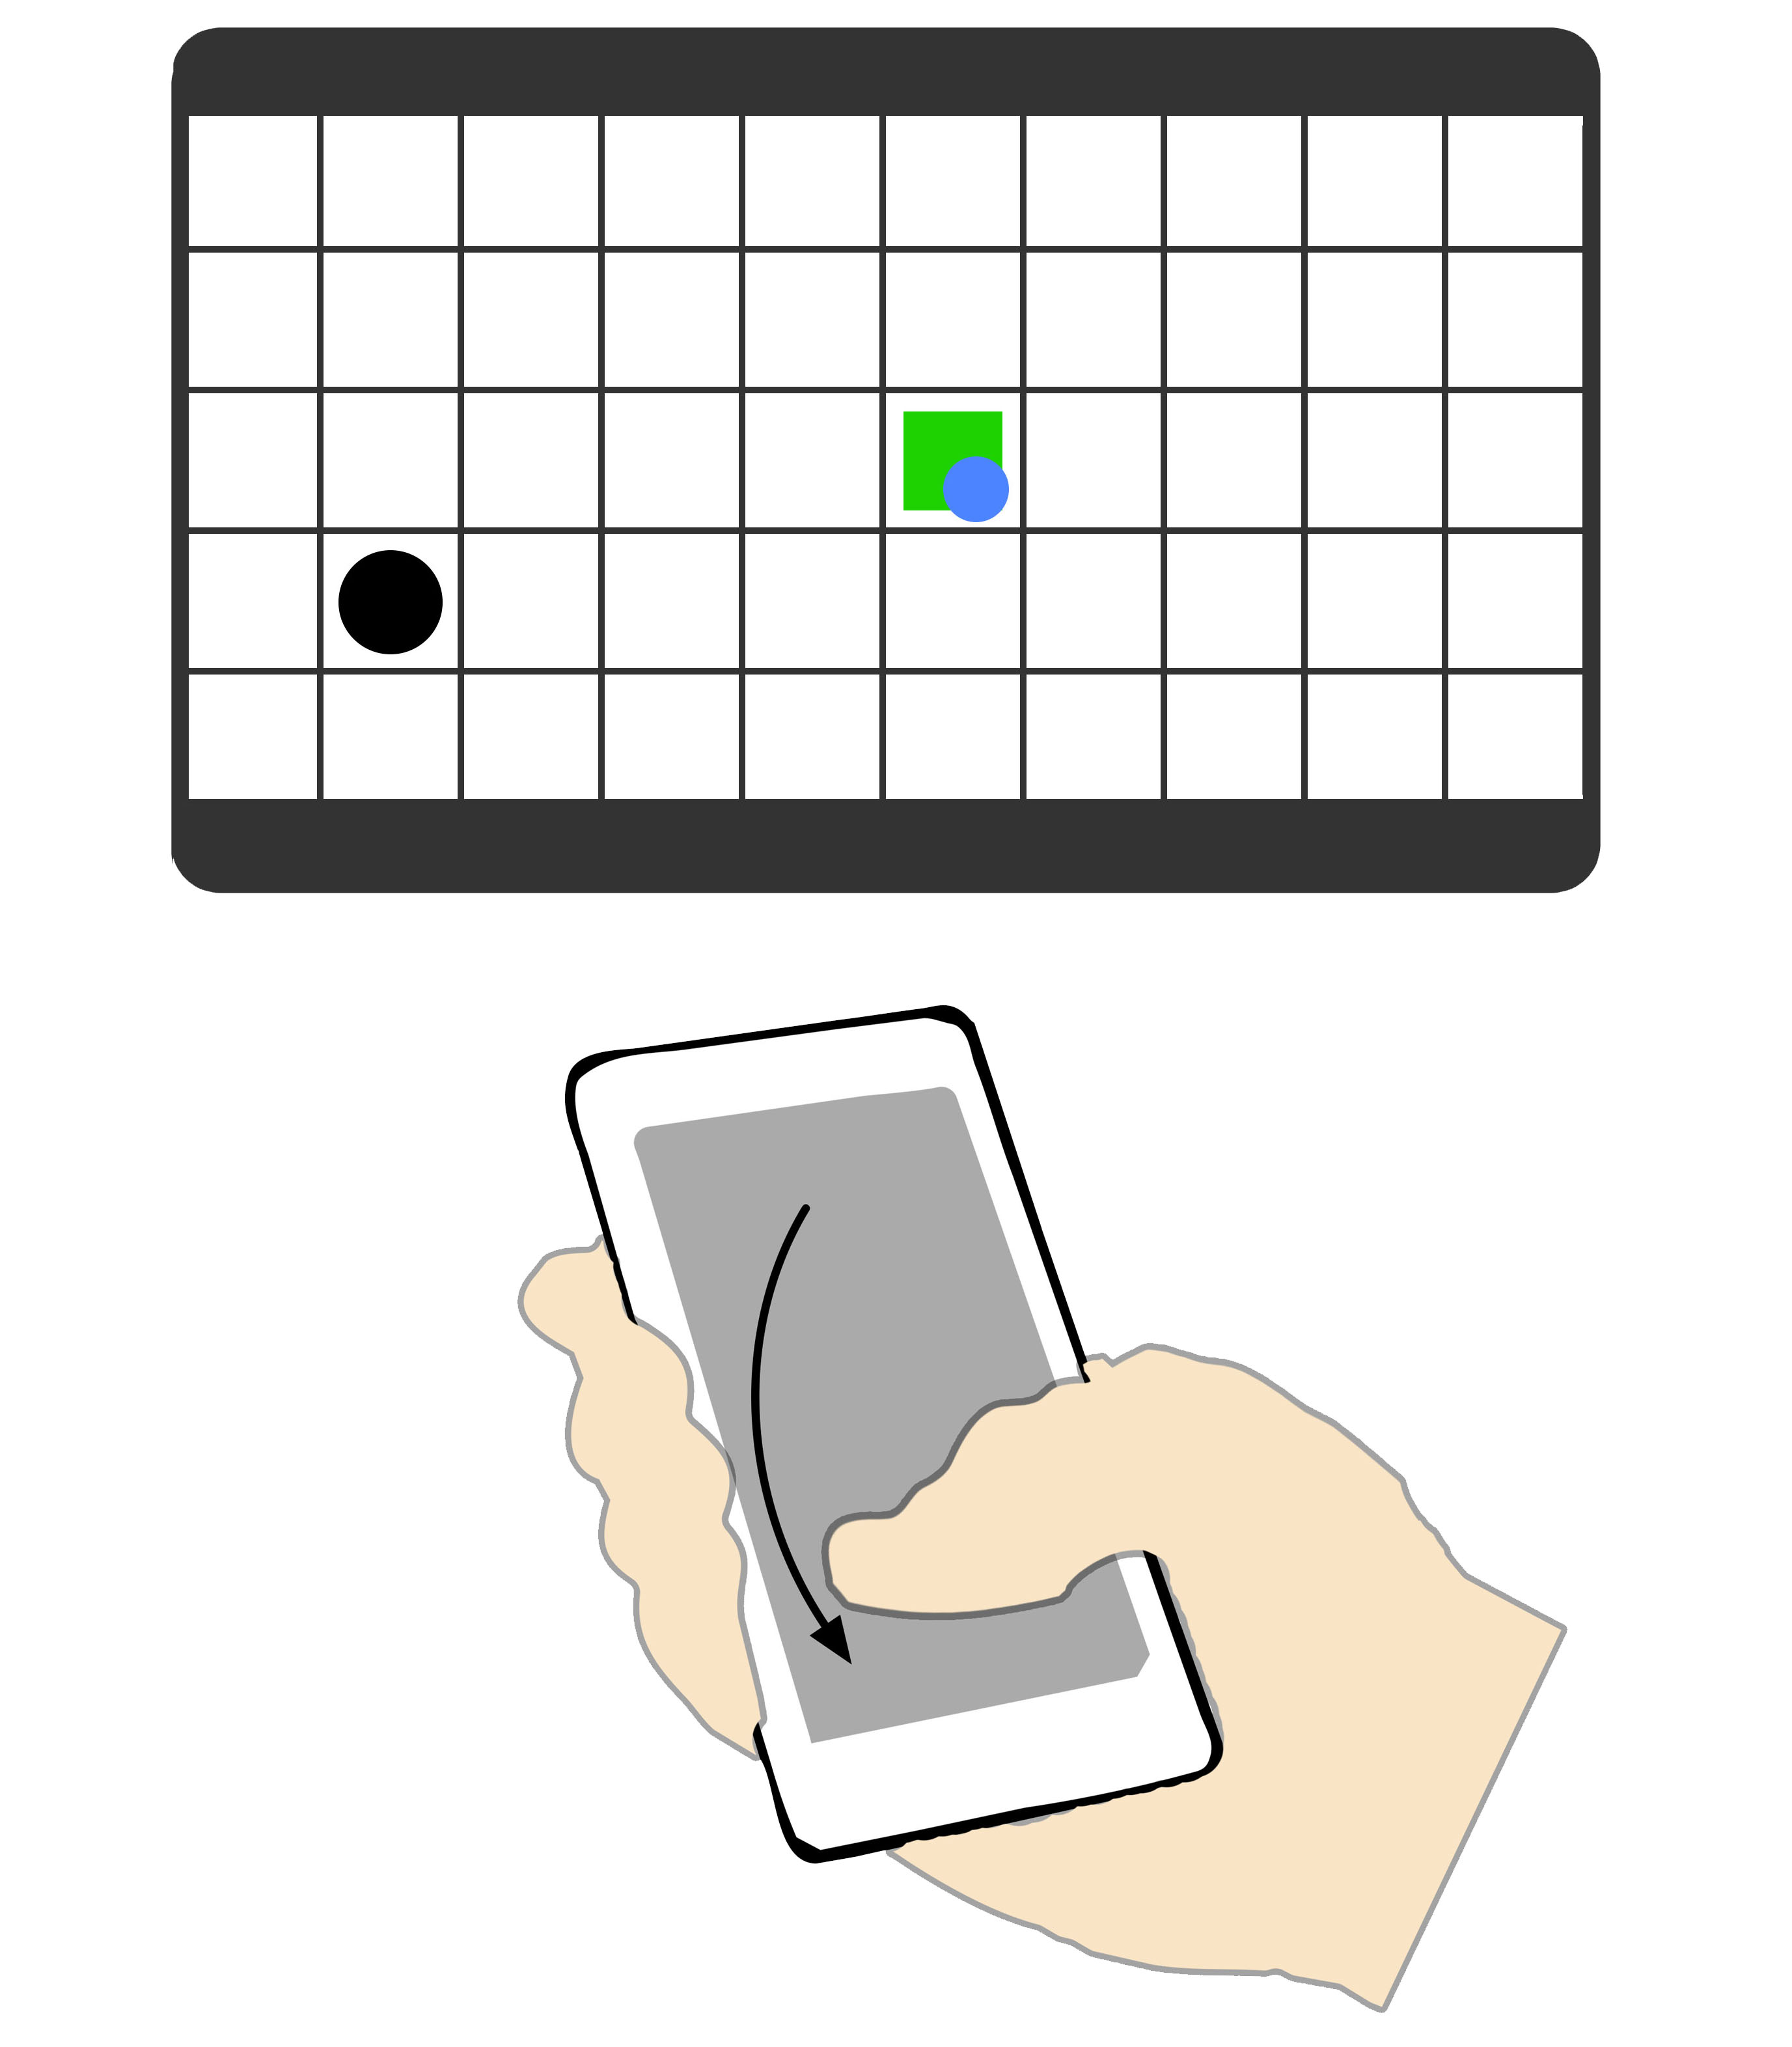
\includegraphics[width = 0.16\columnwidth]{images/techniques/swipePull3.jpg}\label{fig:swipePull3}}\\
	\subfloat[\throw \pull technique]{
		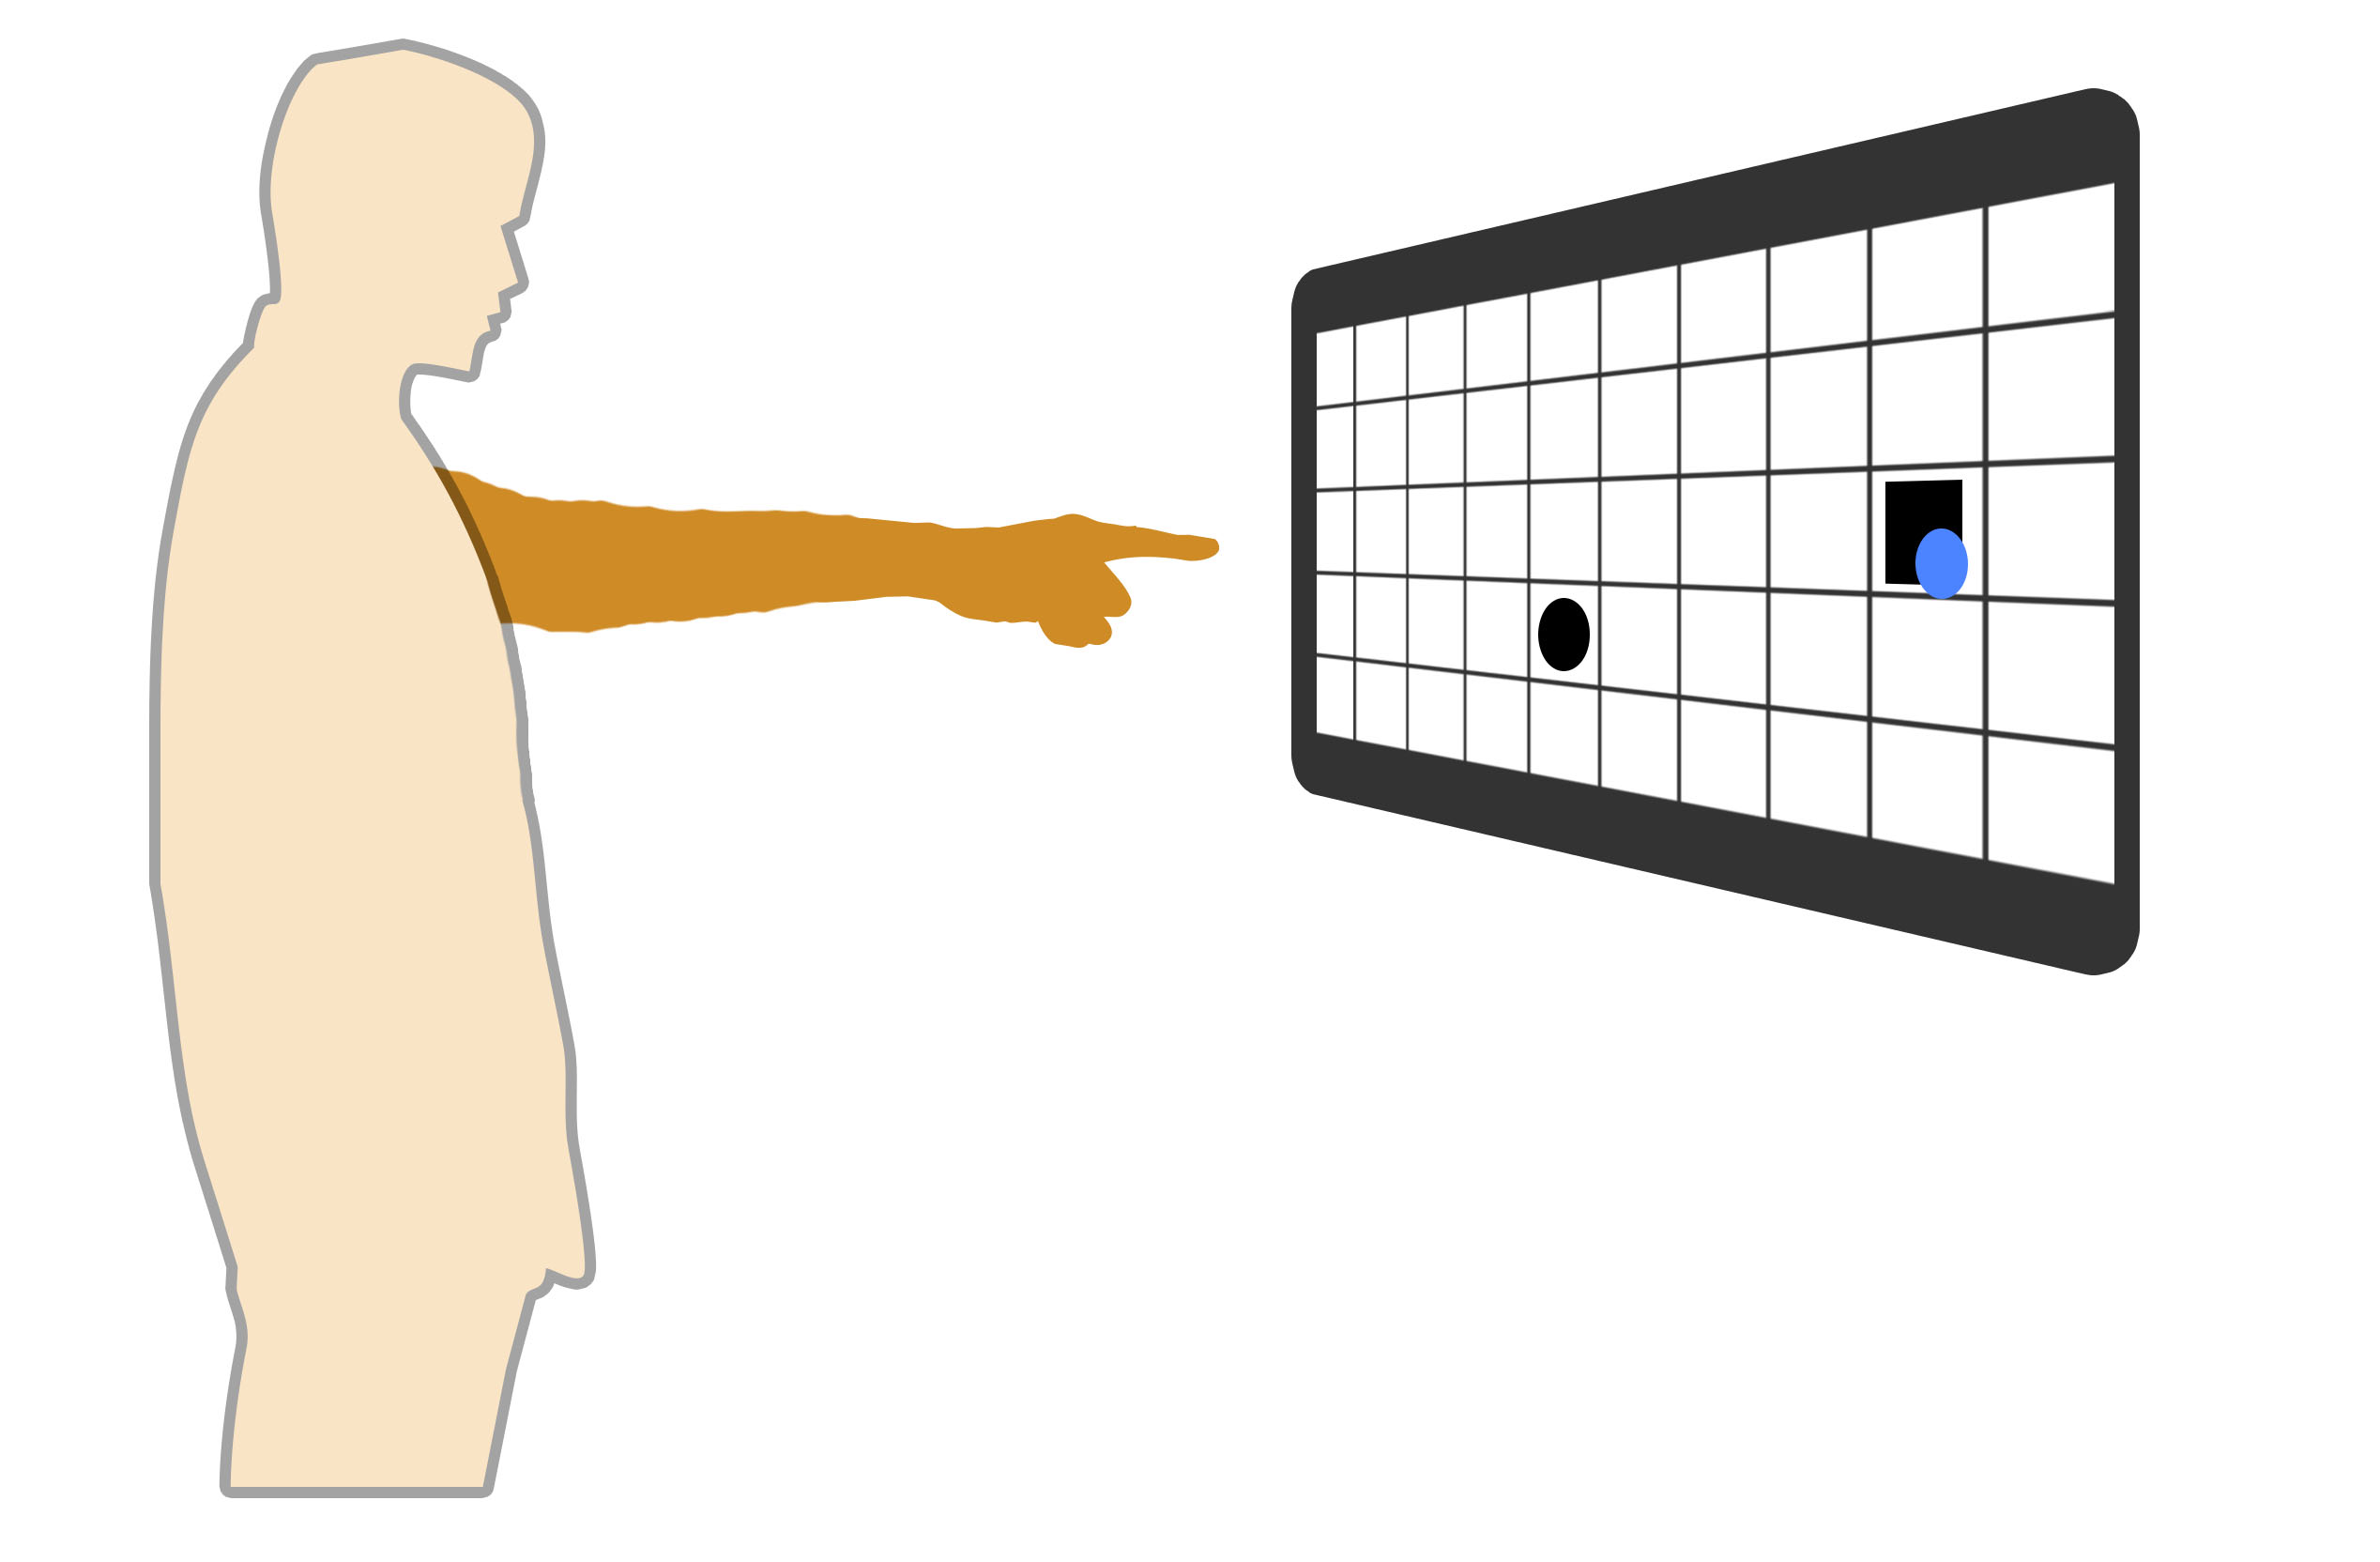
\includegraphics[width = 0.16\columnwidth]{images/techniques/throwPull1.jpg}\label{fig:throwPull1}
		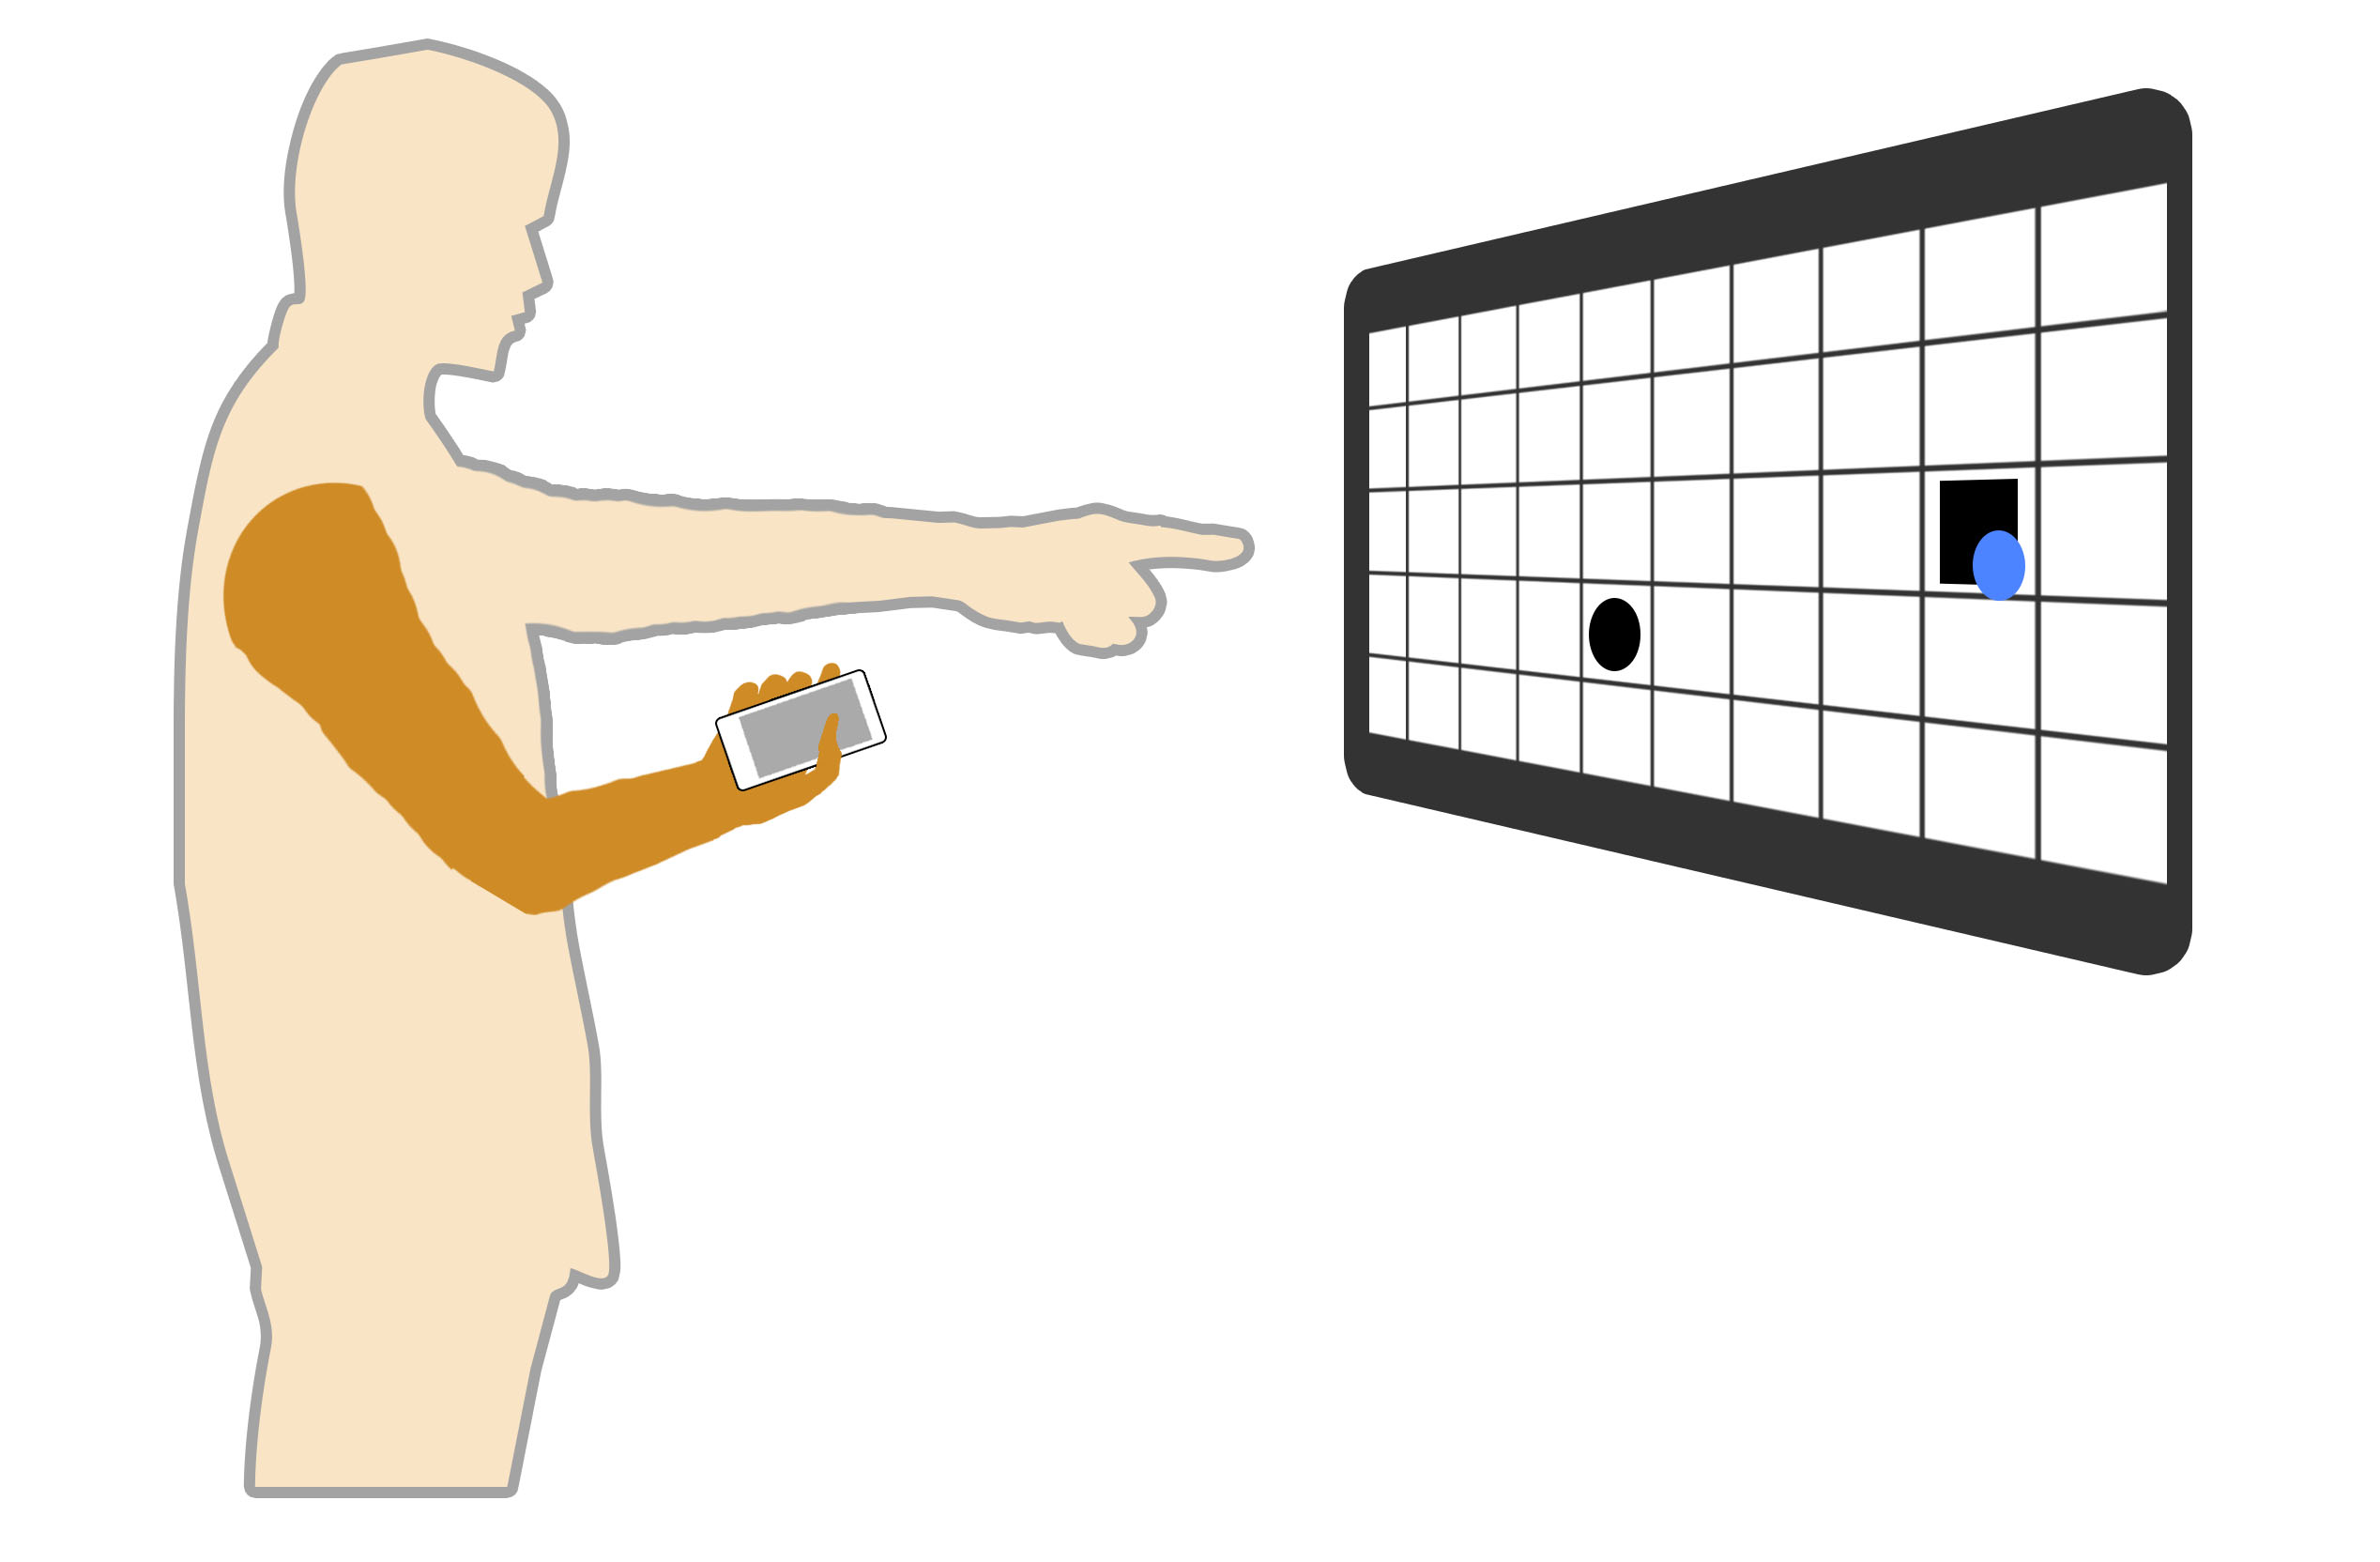
\includegraphics[width = 0.16\columnwidth]{images/techniques/throwPull2.jpg}\label{fig:throwPull2}
		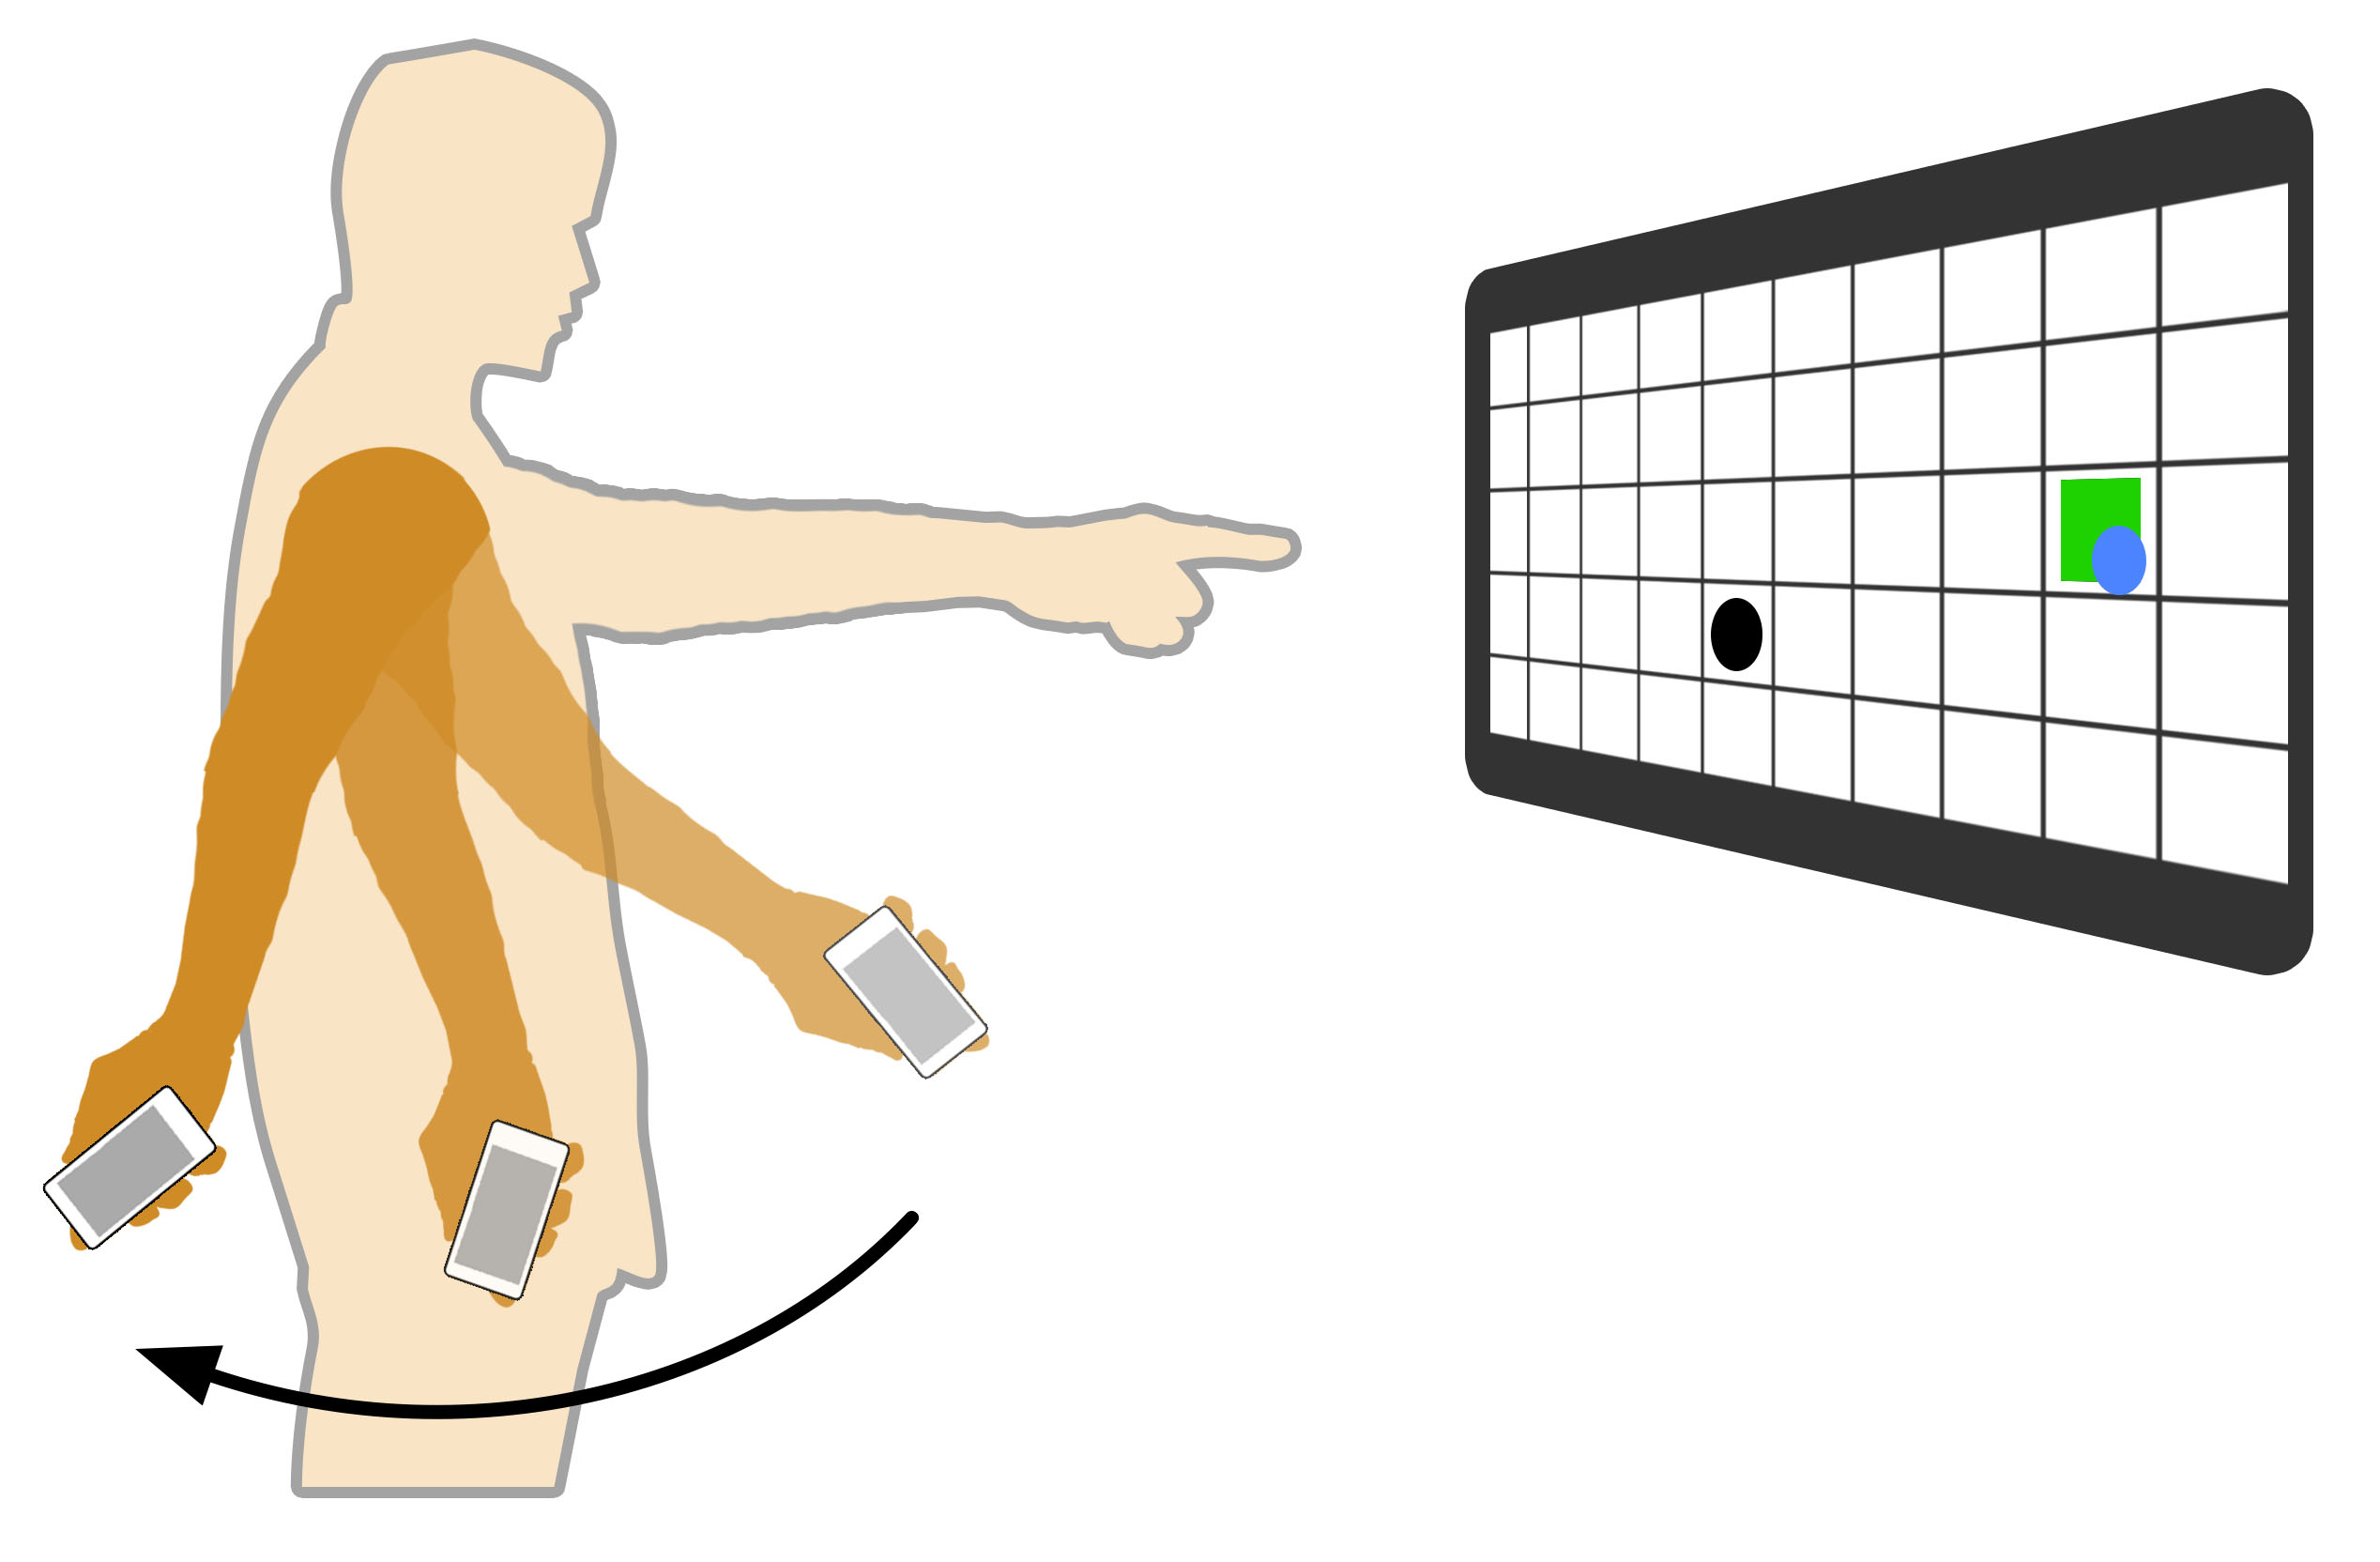
\includegraphics[width = 0.16\columnwidth]{images/techniques/throwPull3.jpg}\label{fig:throwPull3}}
	\subfloat[\tilt \pull technique]{
		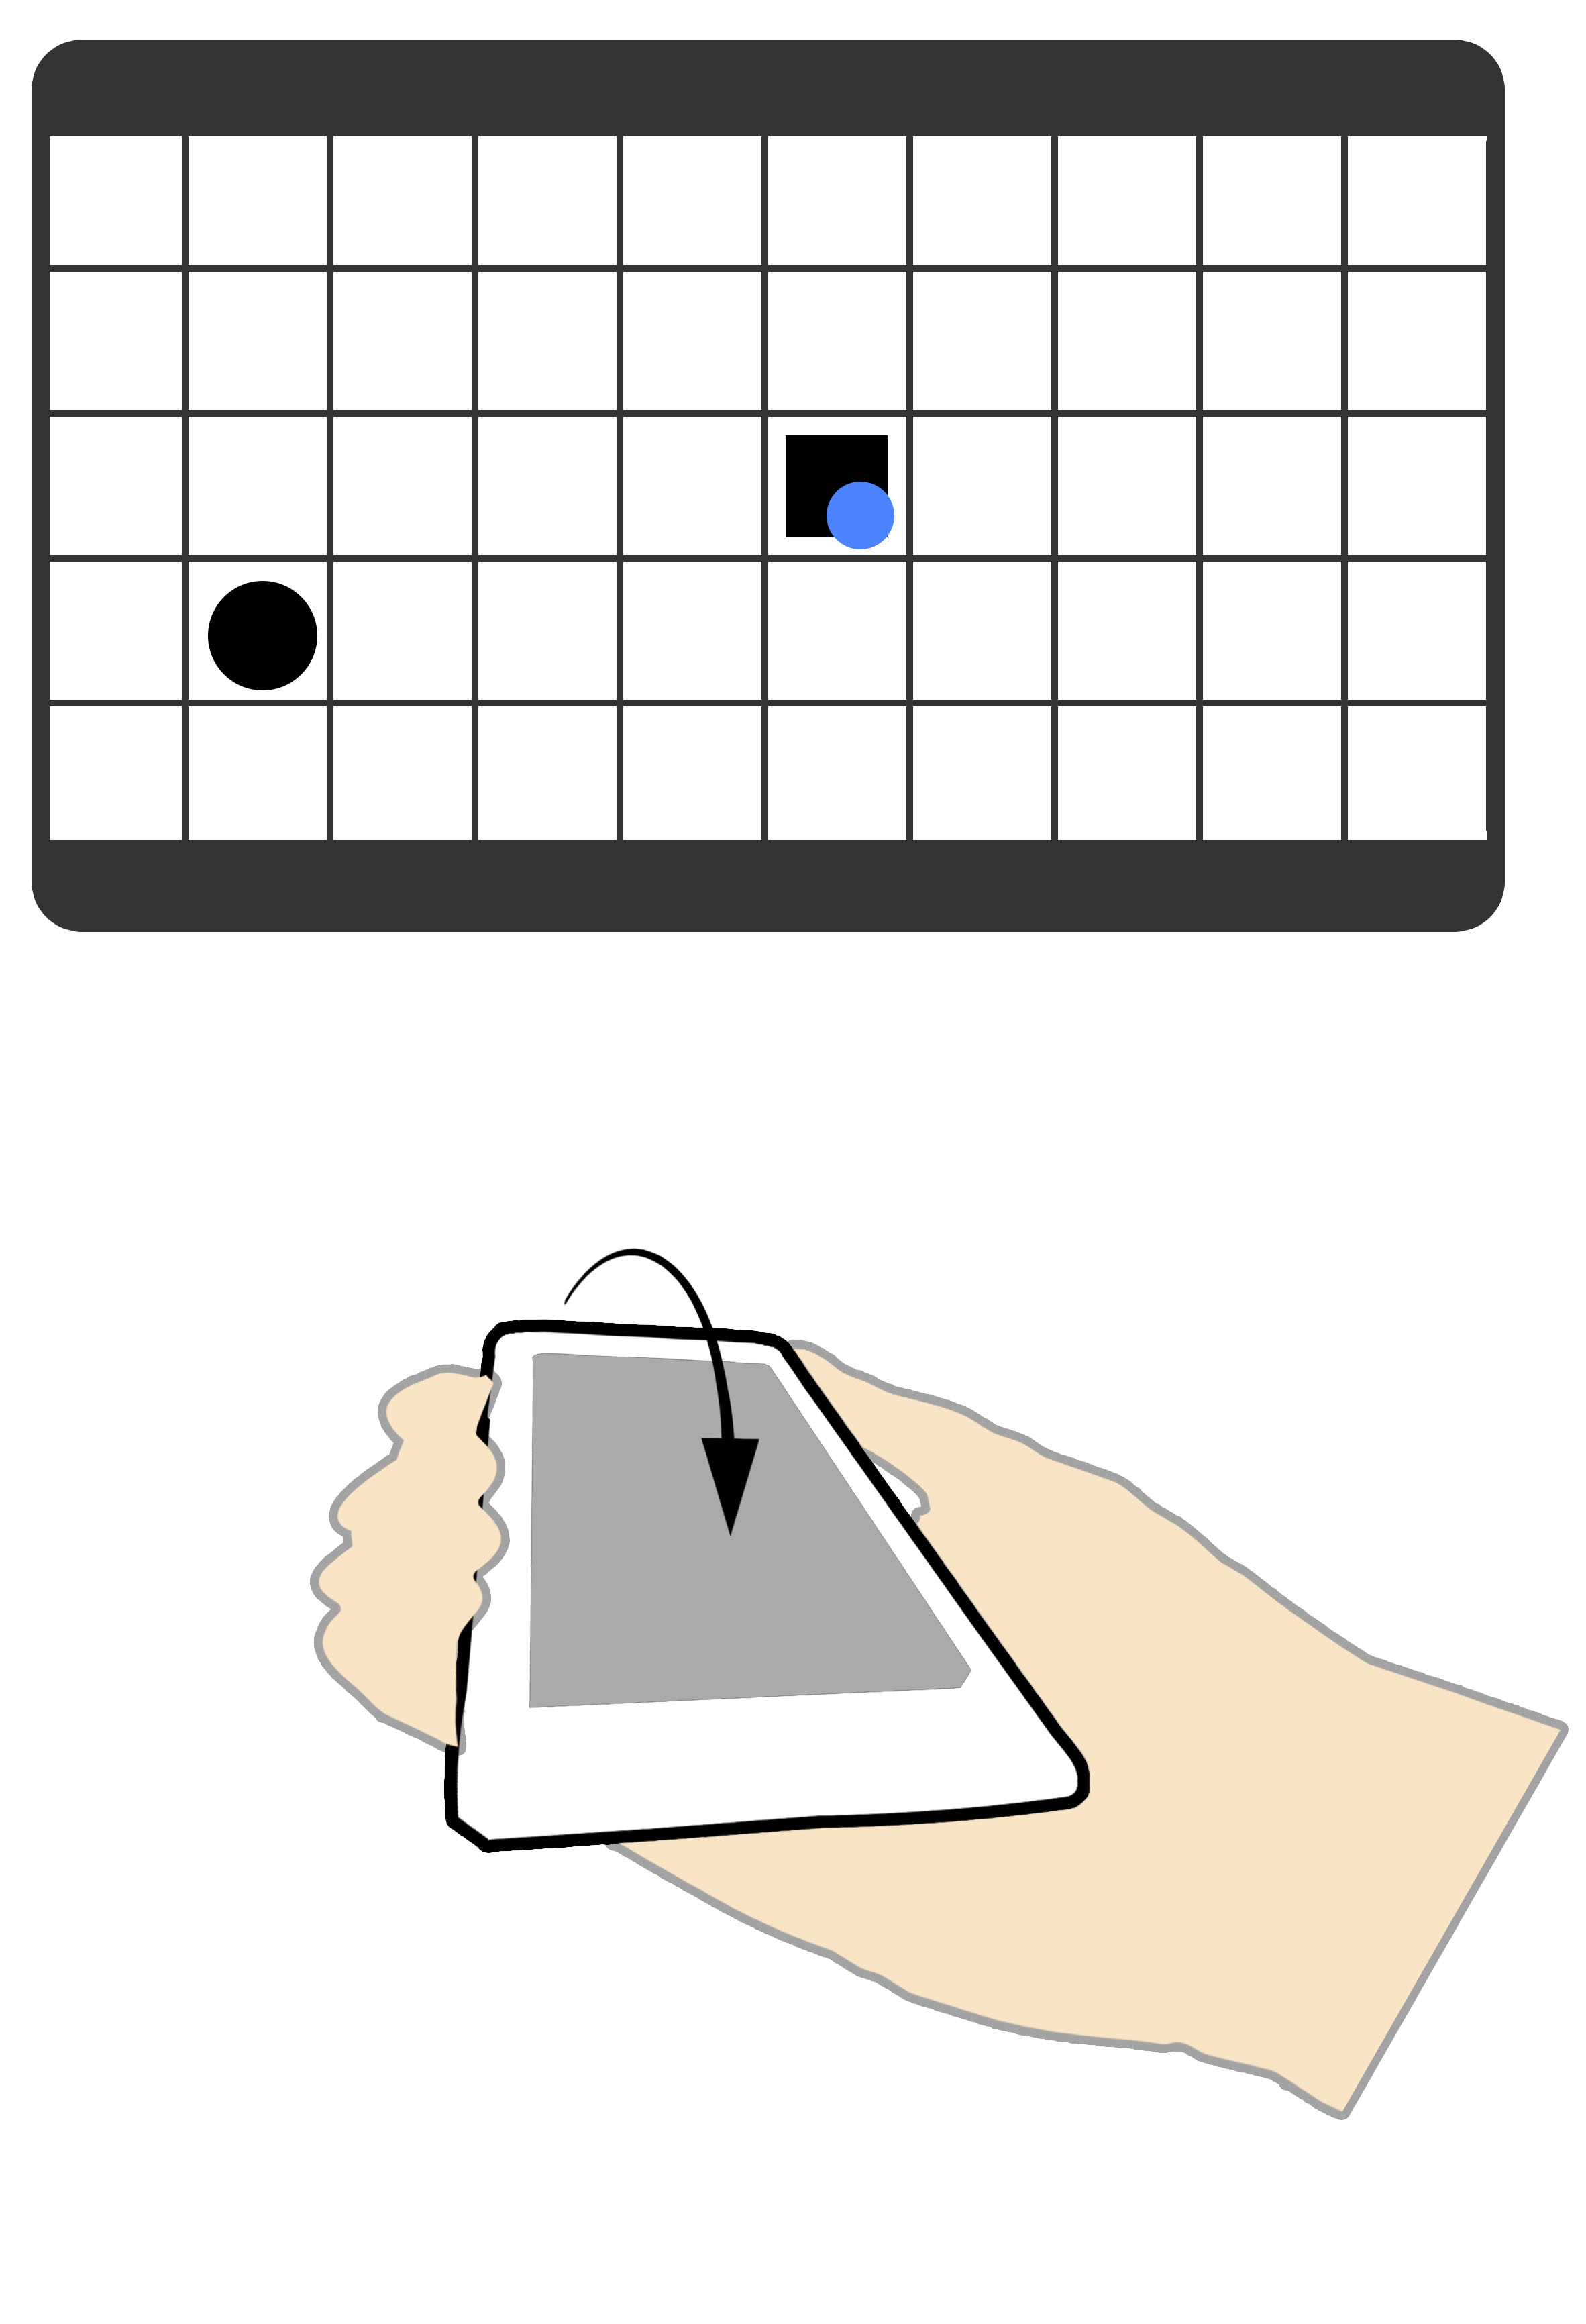
\includegraphics[width = 0.16\columnwidth]{images/techniques/tiltPull1.jpg}\label{fig:tiltPull1}
		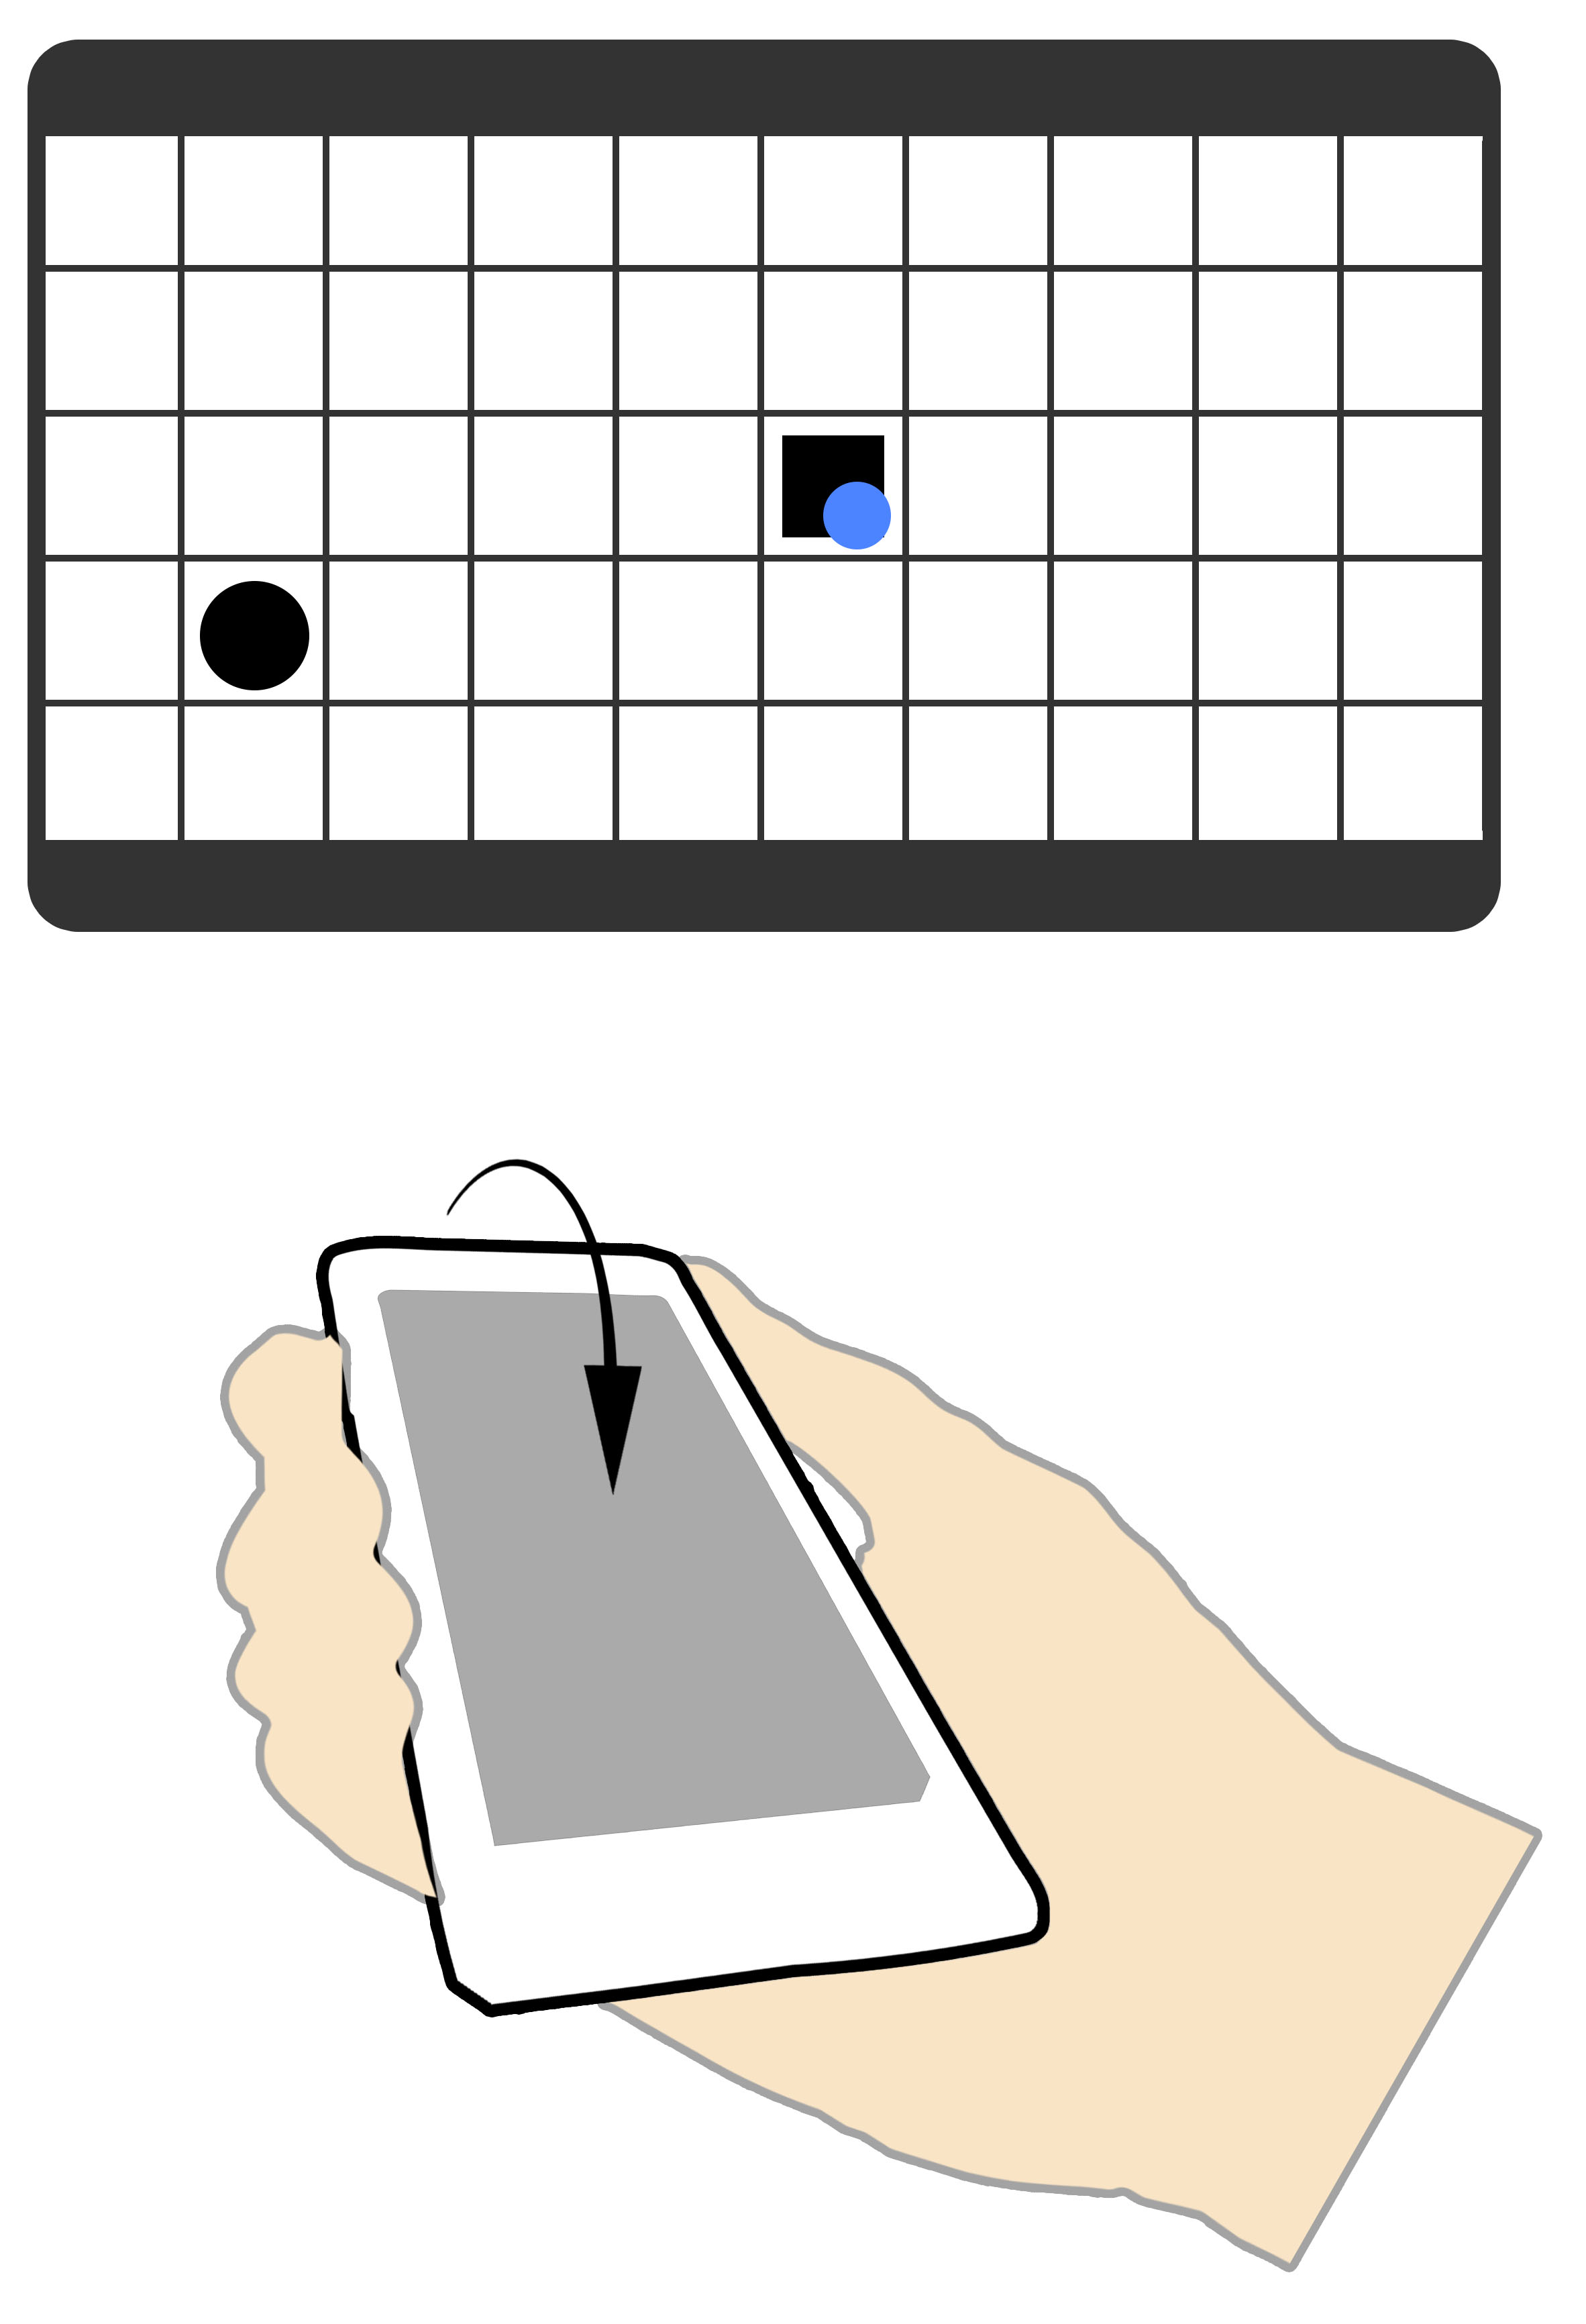
\includegraphics[width = 0.16\columnwidth]{images/techniques/tiltPull2.jpg}\label{fig:tiltPull2}
		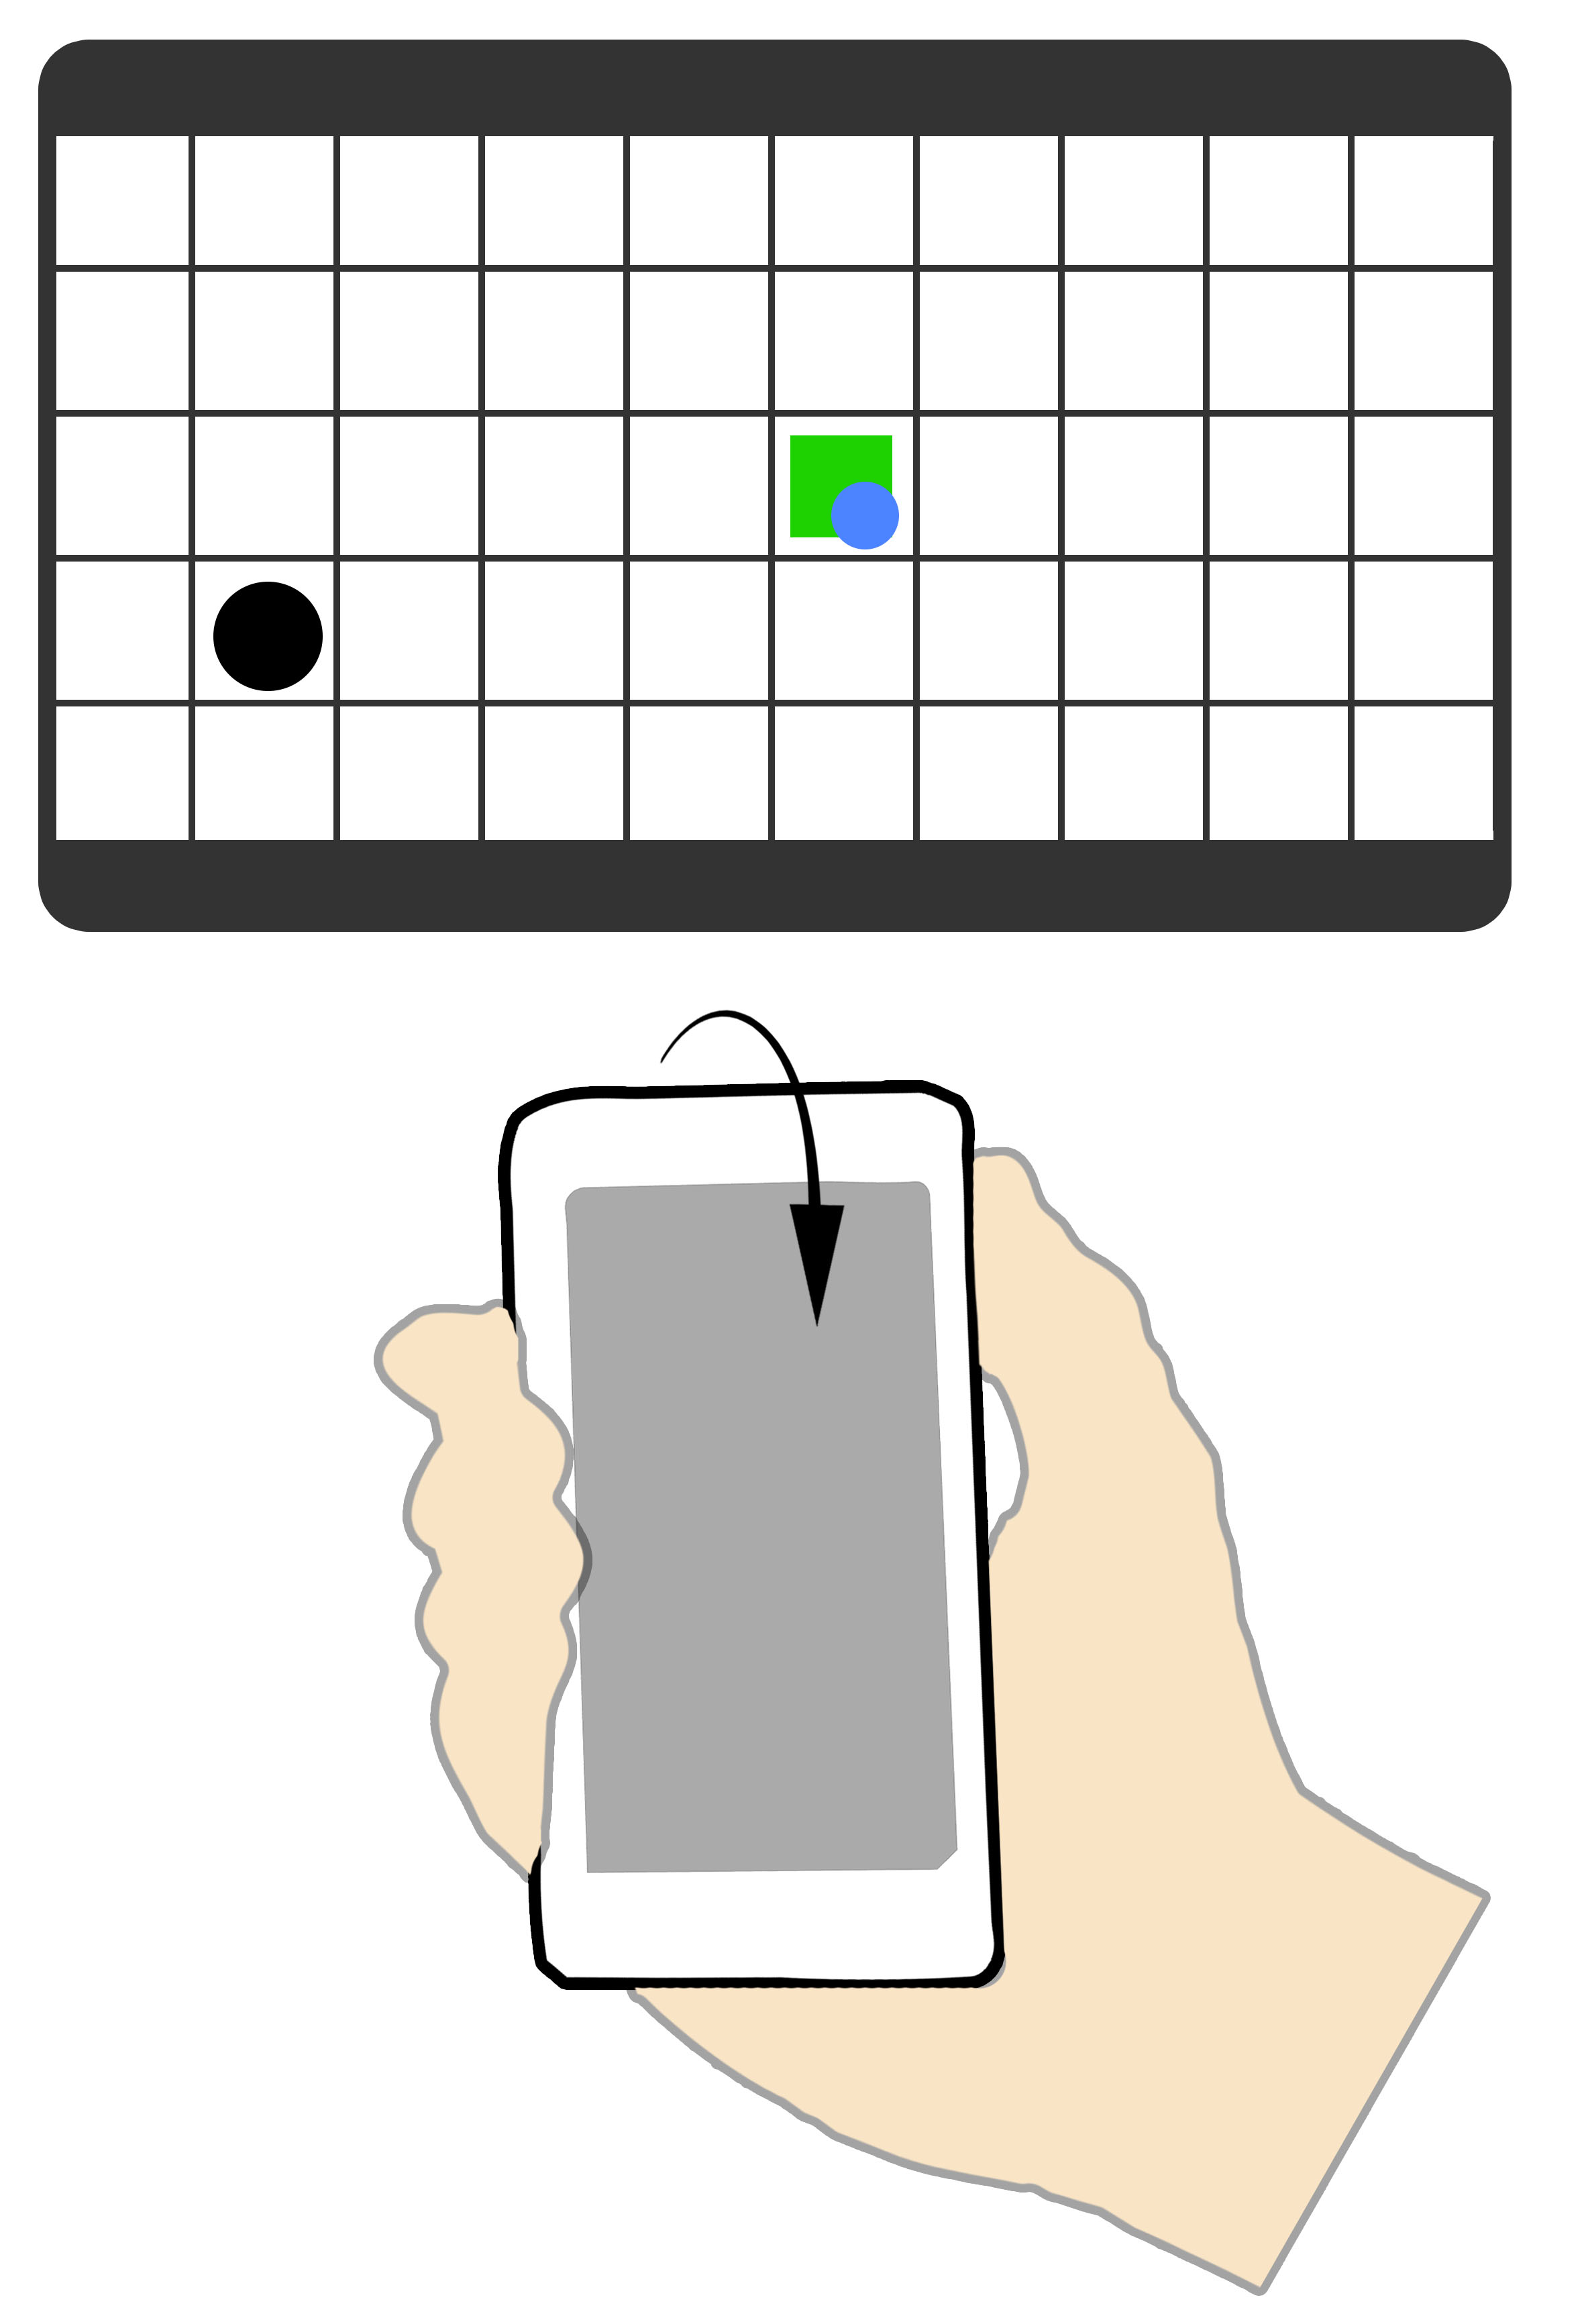
\includegraphics[width = 0.16\columnwidth]{images/techniques/tiltPull3.jpg}\label{fig:tiltPull3}}
	\caption{Illustrations of all the pull techniques that were used in the studies.}
	\label{fig:pullTechniques}
\end{figure}

\subsection*{Improvements to the system}\label{sec:systemImprovements}
We made some improvements to the system compared to last semester, and one of the biggest improvements to the system was to replace the first generation Kinect with the newer Kinect for tracking bodies and detecting hands.
This also meant that we were able to use the Kinect for Windows SDK 2.0 which gives the developer more features for example \textit{``Thumb tracking, end of hand tracking, open and closed hand gestures''}\footnote{\textit{Kinect for Windows SDK 2.0 Features} https://msdn.microsoft.com/library/dn782025.aspx}.

The system will now detect the height from the floor to the head joint and use this in the mapping between a participant's pointing hand and the cursor on the screen.
By doing this we avoid situations from last semester where a participant had to stand on a chair in order to interact with the system.

The implementation and robustness of the techniques have been improved and especially for the \grab, \throw, and \tilt techniques.
The pointing, for all techniques, is much more responsive and without as much jitter as last semester.

The registration of when a hand is opened or closed for \grab \push and \grab \pull is much more robust and does not produce nearly the same amount of false positives as before.
This is both a result of the new Kinect, as well as a much better angle to capture the state of the users hands. 
By lowering the position of the Kinect, instead of having it as close as possible to the large display, the Kinect had a much better overview of the hand.
This meant that it was much more capable of determining the correct state of the hand from what it could see, as the profile of the hand was that much more pronounced.
   
The \throw technique can be performed in an overhand, underhand, or sideways style for both the \pull and \push direction.
This was because we changed the definition of a \throw.
In our first experiment, \throw was defined as a sequence of positions of the hands that needed to be fulfilled. 
In our second experiment, this was scrapped and we defined \throw as a movement from one direction to another (backwards of forwards) of the hands, which had to exceed a certain speed.
This lead to a much more open, as well as more precise, version of the \throw technique. 

We also improved the \tilt technique by improving its interpretation of what a tilting movement was from the readings on the accelerometer. 
While this did lead to considerably less false positives, it did mean that the tilting movement needed to be much more pronounced,.
This was hard for our users, as from our observations, people felt very uncomfortable with the \tilt technique and performed it very slowly, so that they could be as precise as possible with it. 
This would unfortunately not trigger the technique, so users often had to perform it multiple times, each one with slightly more power, until it finally triggered.  


\subsection*{Improvements of the demo videos}\label{sec:videoslastsemester}
When we did the experiment last semester we also had demonstration videos for the participants to look at if they were in doubt of how to perform a certain technique.
The way we did it then was to have the videos run in a loop on the small screen while the test started on the big screen.
Participants were able to start the test even after just seeing the title of the technique they were suppose to do and last semester we saw people jumping straight into it without having looked at the videos of the techniques. 
When this would happen they would simply spend more time in the beginning trying to figure the technique out for themselves.
If they were not successful performing the technique they would finally turn their attention to the demonstration of the technique.
During the experiment some participants noted that they did not notice the video of the technique running in a loop on the small screen.

The quality of the videos we used last semester were not good and people often complained that they were not clear and that they could not clearly see how the technique should be performed.
The videos were shot from two different perspectives and the phone appeared very small on the screen and was not easy to see.
The tempo of the videos and the cuts to white text on black background made the video seem unconnected and possibly a little hard to follow.\\

For this semester we changed the procedure for how we introduced the participants to the techniques and we also changed all the demonstration videos.
The procedure was changed such that participants had to watch the technique being performed two times before the test would start and they could start using the technique themselves.
Another change we made to the procedure were to have the video play on the large screen initially and after two iterations on the large screen the video played in a loop on the small screen.
The videos were changed so they are easier to understand and visibly more clear than were the case previously for example with the interaction on the phone being hard to see.
In the new videos a technique is explained in a slower pace and without cuts to a black screen with white text and we zoomed in on the phone as can be seen in \Cref{fig:demovideC}.
Four screen shots of the Push Throw technique demo video is shown in \Cref{fig:demovideo}.

This lead to a much smoother experience, both for us and the participants.
Last semester, we had to intervene during almost every experiment in order to further explain the techniques for the users.
This time, we very rarely had to intervene and further explain to the participants what they had to do or what they were doing wrong.

\begin{figure}[H]
\subfloat[]{\includegraphics[width = 0.5\columnwidth]{images/demovideo1.pdf}\label{fig:demovideA}}
\subfloat[]{\includegraphics[width = 0.5\columnwidth]{images/demovideo2.pdf}\label{fig:demovideB}}\\
\subfloat[]{\includegraphics[width = 0.5\columnwidth]{images/demovideo3.pdf}\label{fig:demovideC}}
\subfloat[]{\includegraphics[width = 0.5\columnwidth]{images/demovideo4.pdf}\label{fig:demovideD}}
\caption{The images here shows the screen at different times during the demonstration video. The video was shown to the participant before each technique test starts. In \protect\subref{fig:demovideA} the technique is being presented with the direction and the name of the technique. In \protect\subref{fig:demovideB}, \protect\subref{fig:demovideC}, and \protect\subref{fig:demovideD} the video pauses and the participant will be able to read the instructions on the screen.}
\label{fig:demovideo}
\end{figure}

\subsection*{Improvement to the analysis}

In last semester's paper, the results were not cleaned for erroneous attempts which means that we counted all attempts. 
Some attempts would be clear errors such as (1) a participant unintentionally activating a technique with the cursor in a corner of the screen opposite the target, or (2) a participant would spend too much time on an attempt due to system not registering the technique.
These two kind of errors would affect the logged data of distance and time and the statistical method used last semester was also not correct for a within subjects design.
Last semester we also did not have a proper study were we looked at the accuracy of each technique, so our results regarding accuracy are quite misleading. 

Another thing of great importance in regards to the results was that we did not actually perform a correct analysis on the data we generated in our last semester.
As such, our numbers are not correct and we cannot say with confidence if the effects we measured were significant or not. 
We went to much further lengths this semester in order to make sure we performed the correct analysis. 
We consulted regularly with people who had a much larger understanding of statistics, which greatly helped us get the correct model and a much more precise and clear understanding of what the numbers meant. 
This also means that the analysis themselves are correct this time around, and we can say with much certainty that the results we show are, in fact, significant and correct.  
